%\documentclass[PhD]{iitddiss}
%\documentclass[MS]{iitddiss}
% \documentclass[MTech]{iitddiss}
% \documentclass[Dual]{iitddiss}
\documentclass[BTech]{iitddiss}
% \documentclass[Other]{iitddiss}
% IF YOU USE THE OTHER OPTION, THEN YOU MUST FILL OUT THE PROGRAM OPTION BELOW TOO
\program{My Fancy Degree}

% \usepackage{times}
 \usepackage{t1enc}

\usepackage{graphicx}
\usepackage{hyperref} % hyperlinks for references.
\usepackage{amsmath} % easier math formulae, align, subequations \ldots
\usepackage[english]{babel}
\usepackage[utf8]{inputenc}
\usepackage{natbib}
\usepackage{fancyhdr}

\usepackage{booktabs}
\usepackage{multicol}
\usepackage{multirow}
\usepackage{comment}
\usepackage{paralist}
\usepackage{amsfonts}
\usepackage{subcaption}
\usepackage{xcolor}
\usepackage{listings}

 \linespread{1.2}

\pagestyle{fancy}
\renewcommand{\sectionmark}[1]{\markright{\thesection\ #1}}

\fancyhf{}

\rhead{\fancyplain{}{\thepage}} % predefined ()
\lhead{\fancyplain{}{\rightmark}} % 1. sectionname, 1.1 subsection name etc
\cfoot{\textcopyright \text{ } \the\year, \emph{Indian Institute of Technology Delhi}}
\renewcommand{\footrulewidth}{0.4pt}
\begin{document}


%%%%%%%%%%%%%%%%%%%%%%%%%%%%%%%%%%%%%%%%%%%%%%%%%%%%%%%%%%%%%%%%%%%%%%
% Title page

\title{Neural Architectures and Evaluation \\Protocols for Open Information Extraction}

\author{Samarth Aggarwal}
\advisor{Prof. Mausam}
\entrynumber{2016CS10395}
\date{July 2020}
\department{Computer Science and Engineering}

%\nocite{*}
\maketitle

%%%%%%%%%%%%%%%%%%%%%%%%%%%%%%%%%%%%%%%%%%%%%%%%%%%%%%%%%%%%%%%%%%%%%%
% Certificate
\certificate

\vspace*{0.5in}

\noindent This is to certify that the thesis titled {\bf Neural Architectures and Evaluation Protocols for Open Information Extraction}, submitted by {\bf Samarth Aggarwal},
  to the Indian Institute of Technology, Delhi, for
the award of the degree of {\bf Bachelor of Technology}, is a bona fide
record of the research work done by him under our supervision.  The
contents of this thesis, in full or in parts, have not been submitted
to any other Institute or University for the award of any degree or
diploma.

\vspace*{1.5in}

\begin{singlespacing}
\hspace*{-0.25in}
\parbox{2.5in}{
\noindent {\bf Prof.~Mausam} \\
\noindent Professor \\
\noindent Dept. of Physics\\
\noindent IIT-Delhi, 110 016 \\
}
\hspace*{1.0in}
\end{singlespacing}
\vspace*{0.25in}\\
\noindent Place: New Delhi\\
Date: 10th July 2020


%%%%%%%%%%%%%%%%%%%%%%%%%%%%%%%%%%%%%%%%%%%%%%%%%%%%%%%%%%%%%%%%%%%%%%
% Acknowledgements
\acknowledgements

TO BE ADDED

\vspace*{24pt}

\noindent I thank IIT Delhi HPC Facility for compute resources.
\pagebreak

%%%%%%%%%%%%%%%%%%%%%%%%%%%%%%%%%%%%%%%%%%%%%%%%%%%%%%%%%%%%%%%%%%%%%%
% Abstract

\abstract
% \noindent KEYWORDS: \hspace*{0.5em} \parbox[t]{4.4in}{\LaTeX ; Thesis;
%   Style files; Format.}

% \vspace*{24pt}

% \noindent A \LaTeX\ class along with a simple template thesis are
% provided here.  These can be used to easily write a thesis suitable
% for submission at IIT-Delhi.  The class provides options to format
% PhD, MS, M.Tech.\ and B.Tech.\ thesis.  It also allows one to write a
% synopsis using the same class file.  Also provided is a BIB\TeX\ style
% file that formats all bibliography entries as per the IITD format.

% The formatting is as (as far as the author is aware) per the current
% institute guidelines.

%%%%% Abstract = Summary of the entire project %%%%%

%%%%%%%%%%%%%%%%%%%%%%%%%%%%%%%%%%%%%%%%%%%%%%%%%%%%%%%%%%%%%%%%%%
\begin{comment}

  Skelaton

What is OpenIE - 1 line
list a few systems
problems with recent systems
new benchmark was needed
so we made carb, how is carb different
problems with openie models
imojie, mention perf improvements
errors made by imojie, add error analysis
mention mlil paper

\end{comment}
%%%%%%%%%%%%%%%%%%%%%%%%%%%%%%%%%%%%%%%%%%%%%%%%%%%%%%%%%%%%%%%%%%

Open Information Extraction refers to the task of obtaining relation tuples from a sentence. For eg. the sentence ``Donald Trump is the president of United States.'' yields (Donald Trump ; is the president of ; United States) as its OpenIE tuple.

The Open IE paradigm is a useful intermediary for a variety of down-stream tasks such as sentence similarity, event schema induction, text comprehension, knowledge base completion, and more. There have been several attempts at building OpenIE systems that explored rule-based such as OllIE, OpenIE-4 and OpenIE-5. Another wave of OpenIE systems that followed, comprised of neural approaches such as RnnOIE and \citet{cui&al18}. However, the existing openie systems suffer from a wide range of problems. The rule-based systems suffered from cascading errors from a large number of components in succession. The existing neural OpenIE systems, although were able to solve some of these issues to a certain extent, were still far from ideal. Infact, they introduced other problems such as redundancy in their outputs. Together these factors solicit an OpenIE system that is able to overcome the issues pertaining to OpenIE.

Although human inspection revealed that the existing systems were not upto the mark, yet these systems scored high on the existing state-of-the-art OpenIE benchmarks such as OIE2016 \citep{OIE2016}. This means that the existing benchmarks do not correlate well with how humans evaluate OpenIE. In response, we contribute CaRB \citep{bhardwaj&al19}, with a high-quality crowdsourced gold dataset and intuitive evaluation policies that correlate well with human judgement of OpenIE. CaRB establishes itself as the new state of the art OpenIE benchmark.

CaRB evaluation of the \citet{cui&al18}, then state of the art OpenIE systems, confirms its inept performance. We contribute IMoJIE \citep{kolluru&al20}, a neural OpenIE model that outperforms the previous state of the art by about 18 F1 points. It reduces the redundancy in output extractions significantly. Along with it, IMoJIE also presents a novel approach that can be used to generation high-quality training data from multiple low quality datasets.

Although IMoJIE improves the quality of OpenIE tuples significantly, this improvement comes at the cost of speed of extraction. We design a MLIL architecture to overcome the issue of speed of extraction and also obtain further performance nudges from it. This approach also yields a coordination analyzer that significantly improves the yield of the MLIL model.

In the end, we analyse the milestones covered in the world of OpenIE and contribute some ideas for future research.
\pagebreak

%%%%%%%%%%%%%%%%%%%%%%%%%%%%%%%%%%%%%%%%%%%%%%%%%%%%%%%%%%%%%%%%%
% Table of contents etc.

\begin{singlespace}
\tableofcontents
\thispagestyle{empty}

\listoftables
\addcontentsline{toc}{chapter}{LIST OF TABLES}
\listoffigures
\addcontentsline{toc}{chapter}{LIST OF FIGURES}
\end{singlespace}

% The main text will follow from this point so set the page numbering
% to arabic from here on.
\pagenumbering{arabic}

%%%%%%%%%%%%%%%%%%%%%%%%%%%%%%%%%%%%%%%%%%%%%%%%%%%%%%%%%%%%%%%%%%%%%%
% Abbreviations
\abbreviations

\noindent
\begin{tabbing}
xxxxxxxxxxx \= xxxxxxxxxxxxxxxxxxxxxxxxxxxxxxxxxxxxxxxxxxxxxxxx \kill
\textbf{IITD}   \> Indian Institute of Technology, Delhi \\
\textbf{RTFM} \> Read the Fine Manual \\
\end{tabbing}

\pagebreak

%%%%%%%%%%%%%%%%%%%%%%%%%%%%%%%%%%%%%%%%%%%%%%%%%%%%%%%%%%%%%%%%%%%%%%
% Notation

\chapter*{\centerline{NOTATION}}
\addcontentsline{toc}{chapter}{NOTATION}

\begin{singlespace}
\begin{tabbing}
xxxxxxxxxxx \= xxxxxxxxxxxxxxxxxxxxxxxxxxxxxxxxxxxxxxxxxxxxxxxx \kill
\textbf{$r$}  \> Radius, $m$ \\
\textbf{$\alpha$}  \> Angle of thesis in degrees \\
\textbf{$\beta$}   \> Flight path in degrees \\
\end{tabbing}
\end{singlespace}

\pagebreak
\clearpage

% The main text will follow from this point so set the page numbering
% to arabic from here on.
\pagenumbering{arabic}

%%%%%%%%%%%%%%%%%%%%%%%%%%%%%%%%%%%%%%%%%%%%%%%%%%
% Chapters
%%%%%%%%%%%%%%%%%%%%%%%%%%%%%%%%%%%%%%%%%%%%%%%%%%

%%%%%%%%%%%%%%%%%%%%%%%%%%%%%%%%%%%%%%%%%%%%%%%%%%
% Sample Chapter.

\chapter{Sample Chapter}
\label{chap:sample}
This document provides a simple template of how the provided
\verb+iitddiss.cls+ \LaTeX\ class is to be used.  Also provided are
several useful tips to do various things that might be of use when you
write your thesis.

To compile your sources run the following from the command line:
\begin{verbatim}
% pdflatex thesis.tex
% bibtex thesis
% pdflatex thesis.tex
% pdflatex thesis.tex
\end{verbatim}
Modify this suitably for your sources.

To generate PDF's with the links from the \verb+hyperref+ package use
the following command:
\begin{verbatim}
% dvipdfm -o thesis.pdf thesis.dvi
\end{verbatim}

\section{Package Options}

Use this thesis as a basic template to format your thesis.  The
\verb+iitddiss+ class can be used by simply using something like this:
\begin{verbatim}
\documentclass[PhD]{iitddiss}
\end{verbatim}

To change the title page for different degrees just change the option
from \verb+PhD+ to one of \verb+MS+, \verb+MTech+ or \verb+BTech+.
The dual degree pages are not supported yet but should be quite easy
to add.  The title page formatting really depends on how large or
small your thesis title is.  Consequently it might require some hand
tuning.  Edit your version of \verb+iitddiss.cls+ suitably to do this.
I recommend that this be done once your title is final.

To write a synopsis simply use the \verb+synopsis.tex+ file as a
simple template.  The synopsis option turns this on and can be used as
shown below.
\begin{verbatim}
\documentclass[PhD,synopsis]{iitddiss}
\end{verbatim}

Once again the title page may require some small amount of fine
tuning.  This is again easily done by editing the class file.

This sample file uses the \verb+hyperref+ package that makes all
labels and references clickable in both the generated DVI and PDF
files.  These are very useful when reading the document online and do
not affect the output when the files are printed.


\section{Example Figures and tables}

Fig.~\ref{fig:iitd} shows a simple figure for illustration along with
a long caption.  The formatting of the caption text is automatically
single spaced and indented.  Table~\ref{tab:sample} shows a sample
table with the caption placed correctly.  The caption for this should
always be placed before the table as shown in the example.


\begin{figure}[htpb]
  \begin{center}
    \resizebox{50mm}{!} {\includegraphics *{iitd_logo.png}}
    \resizebox{50mm}{!} {\includegraphics *{iitd_logo.png}}
    \caption {Two IITD logos in a row.  This is also an
      illustration of a very long figure caption that wraps around two
      two lines.  Notice that the caption is single-spaced.}
  \label{fig:iitd}
  \end{center}
\end{figure}

\begin{table}[htbp]
  \caption{A sample table with a table caption placed
    appropriately. This caption is also very long and is
    single-spaced.  Also notice how the text is aligned.}
  \begin{center}
  \begin{tabular}[c]{|c|r|} \hline
    $x$ & $x^2$ \\ \hline
    1  &  1   \\
    2  &  4  \\
    3  &  9  \\
    4  &  16  \\
    5  &  25  \\
    6  &  36  \\
    7  &  49  \\
    8  &  64  \\ \hline
  \end{tabular}
  \label{tab:sample}
  \end{center}
\end{table}

\section{Bibliography with BIB\TeX}

I strongly recommend that you use BIB\TeX\ to automatically generate
your bibliography.  It makes managing your references much easier.  It
is an excellent way to organize your references and reuse them.  You
can use one set of entries for your references and cite them in your
thesis, papers and reports.  If you haven't used it anytime before
please invest some time learning how to use it.

I've included a simple example BIB\TeX\ file along in this directory
called \verb+refs.bib+.  The \verb+iitddiss.cls+ class package which
is used in this thesis and for the synopsis uses the \verb+natbib+
package to format the references along with a customized bibliography
style provided as the \verb+iitd.bst+ file in the directory containing
\verb+thesis.tex+.  Documentation for the \verb+natbib+ package should
be available in your distribution of \LaTeX.  Basically, to cite the
author along with the author name and year use \verb+\cite{key}+ where
\verb+key+ is the citation key for your bibliography entry.  You can
also use \verb+\citet{key}+ to get the same effect.  To make the
citation without the author name in the main text but inside the
parenthesis use \verb+\citep{key}+.  The following paragraph shows how
citations can be used in text effectively.

More information on BIB\TeX\ is available in the book by
\cite{lamport:86}.  There are many
references~\citep{lamport:86,sai:16} that explain how to use
BIB\TeX.  Read the \verb+natbib+ package documentation for more
details on how to cite things differently.

Here are other references for example.  \citet{viz:mayavi} presents a
Python based visualization system called MayaVi in a conference paper.
\citet{pan:pr:flat-fst} illustrates a journal article with multiple
authors.  Python~\citep{py:python} is a programming language and is
cited here to show how to cite something that is best identified with
a URL.

\section{Other useful \LaTeX\ packages}

The following packages might be useful when writing your thesis.

\begin{itemize}
\item It is very useful to include line numbers in your document.
  That way, it is very easy for people to suggest corrections to your
  text.  I recommend the use of the \texttt{lineno} package for this
  purpose.  This is not a standard package but can be obtained on the
  internet.  The directory containing this file should contain a
  lineno directory that includes the package along with documentation
  for it.

\item The \texttt{listings} package should be available with your
  distribution of \LaTeX.  This package is very useful when one needs
  to list source code or pseudo-code.

\item For special figure captions the \texttt{ccaption} package may be
  useful.  This is specially useful if one has a figure that spans
  more than two pages and you need to use the same figure number.

\item The notation page can be entered manually or automatically
  generated using the \texttt{nomencl} package.

\end{itemize}

More details on how to use these specific packages are available along
with the documentation of the respective packages.

%%%%%%%%%%%%%%%%%%%%%%%%%%%%%%%%%%%%%%%%%%%%%%%%%%
% Introduction.

\chapter{Introduction}
% Hi this is a sample citation \cite{bhardwaj&al19}.\\
\label{chap:intro}
This document provides a simple template of how the provided
\verb+iitddiss.cls+ \LaTeX\ class is to be used.  Also provided are
several useful tips to do various things that might be of use when you
write your thesis.

To compile your sources run the following from the command line:
\begin{verbatim}
% pdflatex thesis.tex
% bibtex thesis
% pdflatex thesis.tex
% pdflatex thesis.tex
\end{verbatim}
Modify this suitably for your sources.

To generate PDF's with the links from the \verb+hyperref+ package use
the following command:
\begin{verbatim}
% dvipdfm -o thesis.pdf thesis.dvi
\end{verbatim}

\section{Package Options}

Use this thesis as a basic template to format your thesis.  The
\verb+iitddiss+ class can be used by simply using something like this:
\begin{verbatim}
\documentclass[PhD]{iitddiss}
\end{verbatim}

To change the title page for different degrees just change the option
from \verb+PhD+ to one of \verb+MS+, \verb+MTech+ or \verb+BTech+.
The dual degree pages are not supported yet but should be quite easy
to add.  The title page formatting really depends on how large or
small your thesis title is.  Consequently it might require some hand
tuning.  Edit your version of \verb+iitddiss.cls+ suitably to do this.
I recommend that this be done once your title is final.

To write a synopsis simply use the \verb+synopsis.tex+ file as a
simple template.  The synopsis option turns this on and can be used as
shown below.
\begin{verbatim}
\documentclass[PhD,synopsis]{iitddiss}
\end{verbatim}

Once again the title page may require some small amount of fine
tuning.  This is again easily done by editing the class file.

This sample file uses the \verb+hyperref+ package that makes all
labels and references clickable in both the generated DVI and PDF
files.  These are very useful when reading the document online and do
not affect the output when the files are printed.


\section{Example Figures and tables}

Fig.~\ref{fig:iitd} shows a simple figure for illustration along with
a long caption.  The formatting of the caption text is automatically
single spaced and indented.  Table~\ref{tab:sample} shows a sample
table with the caption placed correctly.  The caption for this should
always be placed before the table as shown in the example.


\begin{figure}[htpb]
  \begin{center}
    \resizebox{50mm}{!} {\includegraphics *{iitd_logo.png}}
    \resizebox{50mm}{!} {\includegraphics *{iitd_logo.png}}
    \caption {Two IITD logos in a row.  This is also an
      illustration of a very long figure caption that wraps around two
      two lines.  Notice that the caption is single-spaced.}
  \label{fig:iitd}
  \end{center}
\end{figure}

\begin{table}[htbp]
  \caption{A sample table with a table caption placed
    appropriately. This caption is also very long and is
    single-spaced.  Also notice how the text is aligned.}
  \begin{center}
  \begin{tabular}[c]{|c|r|} \hline
    $x$ & $x^2$ \\ \hline
    1  &  1   \\
    2  &  4  \\
    3  &  9  \\
    4  &  16  \\
    5  &  25  \\
    6  &  36  \\
    7  &  49  \\
    8  &  64  \\ \hline
  \end{tabular}
  \label{tab:sample}
  \end{center}
\end{table}

\section{Bibliography with BIB\TeX}

I strongly recommend that you use BIB\TeX\ to automatically generate
your bibliography.  It makes managing your references much easier.  It
is an excellent way to organize your references and reuse them.  You
can use one set of entries for your references and cite them in your
thesis, papers and reports.  If you haven't used it anytime before
please invest some time learning how to use it.

I've included a simple example BIB\TeX\ file along in this directory
called \verb+refs.bib+.  The \verb+iitddiss.cls+ class package which
is used in this thesis and for the synopsis uses the \verb+natbib+
package to format the references along with a customized bibliography
style provided as the \verb+iitd.bst+ file in the directory containing
\verb+thesis.tex+.  Documentation for the \verb+natbib+ package should
be available in your distribution of \LaTeX.  Basically, to cite the
author along with the author name and year use \verb+\cite{key}+ where
\verb+key+ is the citation key for your bibliography entry.  You can
also use \verb+\citet{key}+ to get the same effect.  To make the
citation without the author name in the main text but inside the
parenthesis use \verb+\citep{key}+.  The following paragraph shows how
citations can be used in text effectively.

More information on BIB\TeX\ is available in the book by
\cite{lamport:86}.  There are many
references~\citep{lamport:86,sai:16} that explain how to use
BIB\TeX.  Read the \verb+natbib+ package documentation for more
details on how to cite things differently.

Here are other references for example.  \citet{viz:mayavi} presents a
Python based visualization system called MayaVi in a conference paper.
\citet{pan:pr:flat-fst} illustrates a journal article with multiple
authors.  Python~\citep{py:python} is a programming language and is
cited here to show how to cite something that is best identified with
a URL.

\section{Other useful \LaTeX\ packages}

The following packages might be useful when writing your thesis.

\begin{itemize}
\item It is very useful to include line numbers in your document.
  That way, it is very easy for people to suggest corrections to your
  text.  I recommend the use of the \texttt{lineno} package for this
  purpose.  This is not a standard package but can be obtained on the
  internet.  The directory containing this file should contain a
  lineno directory that includes the package along with documentation
  for it.

\item The \texttt{listings} package should be available with your
  distribution of \LaTeX.  This package is very useful when one needs
  to list source code or pseudo-code.

\item For special figure captions the \texttt{ccaption} package may be
  useful.  This is specially useful if one has a figure that spans
  more than two pages and you need to use the same figure number.

\item The notation page can be entered manually or automatically
  generated using the \texttt{nomencl} package.

\end{itemize}

More details on how to use these specific packages are available along
with the documentation of the respective packages.

%%%%%%%%%%%%%%%%%%%%%%%%%%%%%%%%%%%%%%%%%%%%%%%%%%
% Literature Survey.

\chapter{Literature Survey}
\label{chap:literature_survey}
\section{Existing OIE Systems}

    The existing OpenIE systems can be broadly categorised into two categories - Rule-Based Systems, and Neural Systems.

    \subsection{Rule-Based Systems}
        Traditional open extractors are rule-based or statistical, e.g., Textrunner \cite{banko&al07}, ReVerb \cite{Fader&al11,etzioni-ijcai11}, OLLIE \cite{Mausam&al12}, Stanford-IE \cite{angeli&al15}, ClausIE \cite{corro&al13}, OpenIE-4 \cite{christensen&al11,pal&al16}, OpenIE-5 \cite{Saha&al2017, Saha2018OpenIE}, PropS \cite{Stanovsky&al2016}, and MinIE \cite{gashteovski&al17}. These systems are largely unsupervised in nature, or bootstrapped from extractions made by earlier systems. They use syntactic or semantic parsers combined with rules to extract tuples from sentences.

        % \subsubsection{ClausIE}
        % \subsubsection{PropS}
        % \subsubsection{OllIE}
        % \subsubsection{OpenIE - 4}
        % \subsubsection{OpenIE - 5}

    \subsection{Neural Systems}
        To bypass error accumulation in rule-based systems with multiple subcomponents, end-to-end neural systems have been proposed recently. They belong to one of two paradigms: sequence \textit{labeling} or sequence \textit{generation}.

        \subsubsection{Sequence Labelling}
            \emph{Sequence Labeling} involves tagging each word in the input sentence as belonging to the subject, predicate, object or other. The final extraction is obtained by collecting labeled spans into different fields and constructing a tuple. RnnOIE \citep{stanovsky&al18} is a labeling system that first identifies the relation words and then uses sequence labelling to get their arguments. It is trained on OIE2016 dataset, which postprocesses SRL data for OpenIE \citep{Stanovsky2016EMNLP}.

            SenseOIE \citep{roy&al19}, improves upon RnnOIE by using the extractions of multiple OpenIE systems as features in a sequence labeling setting. However, their training requires manually annotated gold extractions, which is not scalable for the task. This restricts SenseOIE to train on a dataset of 3,000 sentences. In contrast, our proposed \textit{Score-and-Filter} mechanism is unsupervised and can scale unboundedly. \citet{jiang12019improving} is another labeling system that better calibrates extractions across sentences.
    
            SpanOIE \citep{zhan&al19} uses a span selection model, a variant of the sequence labelling paradigm. Firstly, the predicate module finds the predicate spans in a sentence. Subsequently, the argument module outputs the arguments for this predicate. However, SpanOIE cannot extract nominal relations. Moreover, it bootstraps its training data over a single OpenIE system only.

        \subsubsection{Sequence Generation}
            \emph{Sequence Generation} uses a Seq2Seq model to generate output extractions one word at a time. The generated sequence contains field demarcators, which are used to convert the generated flat sequence to a tuple.
            
            Copy Attention \citep{cui&al18} is a neural generator trained over bootstrapped data generated from OpenIE-4 extractions on a large corpus. During inference, it uses beam search to get the predicted extractions. It uses a fixed-size beam, limiting it to output a constant number of extractions per sentence. Moreover, our analysis shows that CopyAttention extractions severely lack in diversity, as illustrated in Table~\ref{tab:redundancy-example}.
            
            Our analysis of Copy Attention reveals that it suffers from two drawbacks. First, it does not naturally adapt the number of extractions to the length or complexity of the input sentence.  Second, it is susceptible to \emph{stuttering}: extraction of multiple triples bearing redundant information.
            
            These limitations arise because its decoder has no explicit mechanism to remember what parts of the sentence have already been `consumed' or what triples have already been generated. Its decoder uses a fixed-size beam for inference. However, beam search can only ensure that the extractions are not exact duplicates.
        
            \citet{sun2018logician} propose the \emph{Logician} model, a restricted sequence generation model for extracting tuples from Chinese text. Logician relies on coverage attention and gated-dependency attention, a language-specific heuristic for Chinese. Using coverage attention, the model also tackles generation of multiple extractions while being globally-aware. We compare against Logician's coverage attention as one of the approaches for increasing diversity.

        \subsubsection{Comparison}
        Sequence-labeling based models lack the ability to change the sentence structure or introduce new auxiliary words while uttering predictions. For example, they cannot extract \verb|(Trump, is the President of, US)| from \verb|``US President Trump''|, since `is', `of' are not in the original sentence. Also, they assume that all words in one field of the extraction would occur in the same order as they are in the original sentence. But this may not always be ideal. 
    
        On the other hand, sequence-generation models subsume the former type of models. It comes with the added ability to generate words that are not present in the sentence as well as the ability to mutate the sentence structure.

    %%%%%%%%%%%%%%%%%%%%%%%%%%%%%%%%%%%%%%%%%%%%%%%%%%%%%%%%%%%%%%%%%%%%%%%%%%%%%%%%%%%%%%%%%%

\section{Benckmarks}
    To the best of our knowledge, there were three benchmarks systems available for comparing Open IE systems - OIE2016, RelVis and Wire57.

    \subsection{OIE2016}
        The first and the most prominent is OIE2016 \cite{OIE2016}. This has been widely adopted as the standard evaluation framework to test new systems on (e.g., OIE2016 is used by the NST \citep{Nst} and Neural Open IE \citep{cui&al18} systems).  In OIE2016, gold tuples are generated using an automated rule-based system built on top of a QA-SRL dataset \cite{QA-SRL}. In early analysis we find this dataset to be rather noisy. Table \ref{tab:gold_example} illustrates some sample sentences from this gold dateset. These tuples look obviously wrong, and unfit to be in the gold set.

        In addition to the dataset, \citet{OIE2016} release a scorer that compares a set of gold tuples with a set of system tuples to estimate word-level precision and recall. This scorer has been identified to not penalize long extractions. It also does not penalise extractions for misidentifying parts of a relation in an argument slot (or vice versa), leading to trivial systems that score much better than genuine Open IE systems  \cite{Wire57}. We also observe that the scorer compares words all-to-all allowing multiple same words in an extraction to match a corresponding one in the gold. Thus, simply repeating a word in the extraction will give it a high precision score. Finally, the scorer loops over gold tuples in an arbitrary order, and matches them to predicted extractions in a sequential manner. Once a gold matches to a predicted extraction, it is rendered unavailable for any subsequent, potentially better-matched, extraction.

    \subsection{RelVis}
        Another dataset is RelVis \cite{Relvis}, a benchmark that borrows its data from four different datasets including OIE2016. Since OIE2016 forms a major part of this dataset, it has similar issues with noise. Its scorer makes some modifications to OIE2016. However, it does not reward partial coverage of gold tuples, and forces one system prediction to match just one gold. It also does not penalize overlong extractions.
        
    \subsection{Wire57}
        Finally, Wire57 \cite{Wire57} makes further improvements in the scorer. It  penalises overlong extractions and assigns a token-level precision and recall score to all gold-prediction pairs for a sentence. Moreover, it considers all pairs of extractions in its matching phase. However, it still forces one prediction to match just one gold. It also reports just one score for a system, ignoring the confidence values of the individual predictions that make the precision-recall curve of OIE2016 possible. Our scorer is inspired by theirs, with some changes. More importantly, the dataset used in Wire57 is manually curated, but with only 57 sentences, which is too small to suffice as a comprehensive test dataset.
        
%%%%%%%%%%%%%%%%%%%%%%%%%%%%%%%%%%%%%%%%%%%%%%%%%%%%%%%%%%%%%%%%%%%%%%%%%%%%%%%%%%%%%%%%%%%%%%%%
% Uncategorised
%%%%%%%%%%%%%%%%%%%%%%%%%%%%%%%%%%%%%%%%%%%%%%%%%%%%%%%%%%%%%%%%%%%%%%%%%%%%%%%%%%%%%%%%%%%%%%%%




%%%%%%%%%%%%%%%%%%%%%%%%%%%%%%%%%%%%%%%%%%%%%%%%%%%%%%%%%%%%%%%%%%%%%%%%%%%%%%%%%%%%%%%%%%%%%%%%



%%%%%%%%%%%%%%%%%%%%%%%%%%%%%%%%%%%%%%%%%%%%%%%%%%
% CaRB.

\chapter{CaRB - A Crowdsourced Benchmark for Open IE}
\label{chap:carb}
\section{Overview}
    % Problems with Existing Systems
    \subsection{Need for a New Benchmark}
    Traditionally, these systems have been evaluated over small manually curated gold datasets (e.g., \cite{ReVerb1, Ollie}). There are two problems with this approach. One, it is not reliable due to the small size of annotation. Second, it lacks standardization, since there is no single gold dataset over which all systems are evaluated. Moreover, the guidelines to annotate may vary across datasets and annotators. Recently, some standard benchmarks datasets and evaluators have been proposed: OIE2016 \citep{OIE2016}, RelVis \citep{Relvis}, and  Wire57 \citep{Wire57}. Unfortunately, these datasets are either too small or too noisy to meaningfully compare Open IE systems. 

    % CaRB intro
    \subsection{Establishing a new State-of-the-Art}
    In response, we propose a new benchmark system CaRB:  \textbf{C}rowdsourced \textbf{a}utomatic open \textbf{R}elation extraction \textbf{B}enchmark \citep{bhardwaj&al19}, which has a good sized and high quality dataset, along with better evaluation metrics. In order to create this gold dataset, we crowdsource human annotation of extractions using Amazon Mechanical Turk (MTurk) using the same original sentences as OIE2016. Our MTurk task has an automated system for training and qualifying workers, which makes crowdsourcing this annotation feasible.

    Two Open IE experts (authors of this paper) manually annotate 50 random sentences, which are then used as expert ground truth to evaluate the respective tuples in OIE2016's and CaRB's gold datasets  (Tables \ref{tab:token-level},\ref{tab:lexical}). We find that CaRB outperforms OIE2016 by 21 points in precision and 16 points in recall in token level match. This demonstrates that CaRB's gold dataset is significantly more accurate than OIE2016's. Additionally, when evaluating all systems using our benchmark, we notice that CaRB reverses OIE2016's ranking of PropS and ClausIE. Human verification, again through crowdsourcing, verifies that two systems are ranked more accurately by CaRB. We release CaRB's dataset, along with its evaluator as a novel benchmark for further use by research community.\footnote{\texttt{\href{https://github.com/dair-iitd/CaRB}{https://github.com/dair-iitd/CaRB}}}


\section{Crowdsourcing CaRB Dataset}

    To overcome the shortcomings of dataset noise and size, we crowdsource a high-quality gold dataset for Open IE. We ask  workers over Amazon Mechanical Turk (MTurk) to annotate extractions for the 1,282 sentences in dev and test splits of OIE2016. The workers annotate tuples in the form (arg1, rel, arg2), and also annotate location and time attributes for each tuple, when possible. 

    Open IE annotations are not easy to obtain from non-expert workers. To get acceptable quality,  we train workers using a tutorial that doubles up as a qualification test. Their performance in the test is automatically graded. Only workers that pass this are allowed to move on to the main task. The qualification is integrated with the task so that a new worker is served the tutorial and test first, but a qualified worker is directly taken to the main task. This makes the crowdsourcing process scalable. 

    We divide the task of annotating a sentence into three steps: (1) identifying the relation, (2) identifying the arguments for that relation, and (3) optionally identifying the location and time attributes for the tuple.  The training process for the annotators is split into four steps,  each of which focuses on a different guideline for Open IE. These are:

    \begin{enumerate}%[noitemsep]
        \item {\bf Completeness:} The worker must attempt to extract {\em all} assertions from the sentence.
        \item {\bf Assertedness:} Each tuple must be implied by the original sentence.
        \item {\bf Informativeness:} The worker must include the maximum amount of relevant information in an argument.
        \item {\bf Atomicity:} Each tuple must be an indivisible unit. Whenever possible, the worker must extract multiple atomic tuples from a sentence that has conjunctions. 
    \end{enumerate}
    
    We also develop a user-friendly interface for annotating the sentences, which almost eliminates the need for workers to type anything. 
    However, we note that several workers got frustrated in our qualification test, could not understand the task and left the job. However, several good workers completed the task successfully, and annotated significant high-quality data for us.
    
    For sentences involving reporting verbs like {\em said, told, asked,} etc., some systems annotate additional attributional context for every utterance \cite{Ollie}. For this, we create a separate task, so as to prevent workers from being bombarded with all the rules at the same time.

    We post-process the data to remove obvious incorrect annotations, like ones with a missing arg1 or rel. We also follow the convention of ending a relation with a preposition instead of beginning arg2 with one, so all prepositions are shifted to rel.

\section{The CaRB Scorer}

    We now describe CaRB's approach for scoring system predictions against the gold. Instead of greedily matching gold tuples to system tuples in arbitrary order, CaRB creates an all-pair matching table, with each column as system tuple and each row as gold tuple. It computes precision and recall scores between each pair of tuples. Then, for computing overall recall, the maximum recall score is taken in each row, and averaged. By taking the maximum, recall computation matches a gold tuple with the closest system extraction. For computing precision, the system predictions are matched one to one with gold tuples, in the order of best match score to worst. The match precision scores are then averaged to compute precision.  To compute precision-recall curve this computation is done at different confidence thresholds of system extractions.

    \begin{table}[h]
        {\small
        \centering
        \begin{tabular}{|l|l|l|l|} 
        \hline
        Sentence & \begin{tabular}[c]{@{}l@{}}{\em I ate an apple}\\ {\em and an orange.}\end{tabular}         & \multicolumn{1}{l}{(prec,rec)} &           \\ 
        \hline
        Gold     & \begin{tabular}[c]{@{}l@{}}(I; ate; an apple)\\(I; ate; an orange)\end{tabular} & OIE2016                        & CaRB      \\ 
        \hline
        System 1 & \begin{tabular}[c]{@{}l@{}}(I; ate; an apple\\ and an orange)\end{tabular}      & (1,0.5)                        & (0.57,1)  \\ 
        \hline
        System 2 & (I; ate; an apple)                                                              & (1,0.5)                        & (1,0.87)  \\
        \hline
        \end{tabular}
        \caption{One-to-One Match vs. Multi Match}
        \label{tab:one2one_vs_multi_match}
        }
    \end{table}

    In this way, CaRB's recall computation uses the notion of {\em multi-match}, wherein a gold tuple can match multiple system extractions. This is helpful in avoiding penalizing a system very heavily if it stuffs information from multiple gold tuples in a single extraction. Table \ref{tab:one2one_vs_multi_match} displays an example wherein system 1 combines information from two gold tuples in a single extraction, and system 2 only extracts one of the gold tuples. One-to-one match (OIE2016) is indifferent between the two which means that for OIE2016, adding more information in the same extraction has no value at all. However, multi match (CaRB) assigns higher recall to system 1, since it contains strictly more information, and higher precision to system 2, since its prediction exactly matched a gold extraction. 

    On the other hand, CaRB uses {\em single match} for precision. This is because CaRB’s gold tuples are atomic, and cannot be further divided into more tuples. By single matching for precision, CaRB penalizes Open IE systems that produce several very similar and redundant extractions.

    Another significant change from OIE2016 scorer is in the use of {\em tuple match} instead of {\em lexical match}. CaRB matches relation with relation, and arguments with arguments, however OIE2016 serialized the tuples into a sentence and just computed lexical matches. 
    
    \begin{table}[h]
        \centering
        {\small
        \begin{tabular}{|l|l|l|l|} 
        \hline
        Sentence & {\em I ate an apple.}    & \multicolumn{1}{l}{(prec,rec)} &        \\ 
        \hline
        Gold     & (I; ate; an apple) & OIE2016                        & CaRB   \\ 
        \hline
        System 1 & (I; ate; an apple) & (1,1)                          & (1,1)  \\ 
        \hline
        System 2 & (ate; an apple; I) & (1,1)                          & (0,0)  \\
        \hline
        \end{tabular}
        \caption{Tuple Match vs. Lexical Match}
        \label{tab:tuple_vs_lexical_match}
        }
        \vspace*{-2ex}
    \end{table}

    Table \ref{tab:tuple_vs_lexical_match} illustrates an example when the arguments are shuffled, lexical match (OIE2016) shows no effect but tuple match (CaRB) rightfully decreases the scores. To avoid spurious matches, CaRB considers only matches with atleast one common word in the relation field.

    Finally, some Open IE systems extract n-ary tuples and others do not. To treat all systems on equal footing, we follow previous work and append all higher numbered arguments into arg2. 

\section{Evaluation}
    \subsection{Dataset Quality}

        We first estimate the overall quality of the crowdsourced dataset. To this end, two authors of this paper annotate 50 dev sentences from OIE2016 to create an expert dataset. They first independently annotate tuples from these sentences, achieving an agreement F1 score of 83. They then resolve the differences and  merge these independent sets. This is taken as an expert gold against which both OIE2016 and CaRB datasets are assessed. 

        \begin{table}[h!]
        \centering
        \begin{tabular}{|c|c|c|c|}
        \hline
        Dataset       & Precision & Recall & F1    \\ \hline
        OIE2016 & 0.65     & 0.55  & 0.60 \\ %\hline
        CaRB         & 0.87     & 0.71  & 0.78 \\ \hline
        \end{tabular}
        \vspace*{-1ex}
        \caption{Data quality using token-level match}
        \label{tab:token-level}
        \end{table}
        
        \begin{table}[h]
        \vspace*{-1ex}
        \centering
        \begin{tabular}{|c|c|c|c|}
        \hline
                & Precision & Recall & F1   \\ \hline
        OIE2016 & 0.67      & 0.51      & 0.57 \\ %\hline
        CaRB   & 0.74      & 0.73      & 0.73 \\ \hline
        \end{tabular}
        \vspace*{-1ex}
        \caption{Data quality using lexical match}
        \label{tab:lexical}
        \vspace*{-1ex}
        \end{table}
        
        % OIE2016 Gold vs CaRB Gold
        \begin{table*}[t!]
            \centering
            \begin{tabular}{|l|l|} 
            \hline
            Sent. \# 1 & \textit{ Butters Drive in the Canberra suburb of Phillip is named in his honour . }                                                                                                                                                                                                                                                                                                                         \\ 
            \hline
            OIE2016    & \begin{tabular}[c]{@{}l@{}}( in the Canberra suburb of Phillip is named in his honour . ; drive; ),\\ ( Butters Drive in the Canberra suburb of Phillip ; named ; his honour ) \end{tabular}                                                                                                                                                                                                                \\ 
            \hline
            CaRB       & \begin{tabular}[c]{@{}l@{}}( Butters Drive in the Canberra suburb of Phillip ; is named ; in his honour),\\( Butters Drive ; is ; in the Canberra suburb of Phillip ) \end{tabular}                                                                                                                                                                                                                         \\ 
            \hhline{|==|}
            Sent. \# 2 & \begin{tabular}[c]{@{}l@{}}\textit{ It was only incidentally that economic issues appeared in nationalist}\\\textit{political forms . }\end{tabular}                                                                                                                                                                                                                                                        \\ 
            \hline
            OIE2016    & ( incidentally ; appeared ; economic issues ; nationalist political forms . )                                                                                                                                                                                                                                                                                                                               \\ 
            \hline
            CaRB       & (economic issues ; appeared only incidentally in ; nationalist political forms)                                                                                                                                                                                                                                                                                                                             \\ 
            \hhline{|==|}
            Sent. \# 3 & \begin{tabular}[c]{@{}l@{}}																		\textit{The main reason for this adoption over mainline gimp was its support for }\\\textit{high bit depths which can be~required for film work . }\end{tabular}                                                                                                                                                                                               \\ 
            \hline
            OIE2016    & ( high bit depths ; required ; film work )                                                                                                                                                                                                                                                                                                                                                                  \\ 
            \hline
            CaRB       & \begin{tabular}[c]{@{}l@{}}( this adoption ; has support for ; high bit depths ),\\( high bit depths ; can be required for ; film work ),\\ ( this adoption ; was over ; mainline gimp ),\\( mainline gimp ; has no support for ; high bit depths ),\\ ( its support for high bit depths which can be required for film work ;\\was The main reason for ; this adoption over mainline gimp ) \end{tabular}  \\ 
            \hhline{|==|}
            Sent. \# 4 & \begin{tabular}[c]{@{}l@{}}																		\textit{The number of ones equals the number of zeros plus one , since the state }\\\textit{containing only zeros can not occur .~}									 \end{tabular}                                                                                                                                                                                                     \\ 
            \hline
            OIE2016    & \begin{tabular}[c]{@{}l@{}}( The number of ones ; equals ; the number of zeros plus one ; \\since the state containing only zeros can not occur ),\\( the state ; containing ; only zeros ),\\( the state containing only zeros ; occur ) \end{tabular}                                                                                                                                                     \\ 
            \hline
            CaRB       & \begin{tabular}[c]{@{}l@{}}( The number of ones ; equals ; the number of zeros plus one ),\\ ( the state containing only zeros ; can not occur ) \end{tabular}                                                                                                                                                                                                                                              \\
            \hline
            \end{tabular}
            \caption{Sample gold annotations for OIE2016 vs. CaRB}
            \label{tab:gold_example}
        \end{table*}

        Tables  \ref{tab:token-level} and \ref{tab:lexical} estimate dataset quality of OIE2016 and CaRB. We find that CaRB has enormously high precision and recall values, suggesting that it is a much cleaner dataset. Table \ref{tab:gold_example} compares the crowd sourced annotations and OIE2016 gold annotations for some sample sentences. While there is still scope for improvement, CaRB dataset appears much better than the OIE2016's gold.

        \citet{OIE2016} remark that their gold dataset reaches an F1 of 95.8 on their expert annotation, whereas our assessment suggest values around 60. We surmise that this discrepancy is due to the different gold-prediction scoring schemes used. In original OIE2016 paper, the authors ``match an automated extraction with a gold proposition if both agree on the grammatical head of all of their elements (predicate and arguments)".\footnote{This scheme is later changed in their github  repository to a lexical match, where if the fraction of words in the prediction also present in the gold is above a threshold, the pair is declared a match.} The head match criterion is a much laxer scheme than ours and can explain the very high F1 score against their expert annotation.

    \subsection{Comparison of Open IE Systems}
        % Performance of OpenIE systems on CaRB
        \begin{table}[h!]
        %\vspace*{-1ex}
        \centering
        \begin{tabular}{|l|c|c|c|c|}
        \hline
        System  & Precision & Recall & F1 & AUC  \\ \hline
        % Stanford & {\bf 0.73}      & 0.28      & 0.41 & 0.24 \\ %\hline
        % Ollie       & 0.575          & 0.391          & 0.465 & 0.272 \\ %\hline
        % PropS       & 0.492          & 0.556          & 0.522 & 0.310 \\ %\hline
        % OpenIE 4    & {\bf 0.618}    & 0.515          & \bf{0.562} & \bf{0.351}\\ %\hline
        % OpenIE 5    & 0.604          & 0.521          & 0.559 & 0.349\\ %\hline
        % ClausIE     & 0.508          & \bf{0.593}     & 0.548 & 0.340\\ \hline
        
        Ollie       & 0.505          & 0.346          & 0.411 & 0.224 \\ %\hline
        PropS       & 0.340          & 0.300          & 0.319 & 0.126 \\ %\hline
        OpenIE 4    & {\bf 0.553}    & 0.437          & \bf{0.488} & \bf{0.272}\\ %\hline
        OpenIE 5    & 0.521          & 0.424          & 0.467 & 0.245\\ %\hline
        ClausIE     & 0.411          & \bf{0.496}     & 0.450 & 0.224\\ \hline
        \end{tabular}
        \vspace*{-1ex}
        \caption{Performance of Open IE systems on CaRB}
        \vspace*{-2ex}
        \label{tab:carb}
        \end{table}

        We test the different Open IE systems depicted in \citet{OIE2016}, using the CaRB dataset and scorer. The p-r curves obtained using OIE2016 and CaRB are outlined in figures \ref{fig:pr_oie16} (reproduced from \citet{Rnnoie}) and \ref{fig:pr_carb}. Precision, recall and F1 scores (at max F1 point) and area under precision-recall curve are reported in Table \ref{tab:carb}. It can be seen that the curve for PropS lies above ClausIE at all times in OIE2016, but PropS performs the worse of all systems in CaRB. To verify that CaRB indeed gives the correct ranking, we turn back to human verification.

        % PR_oie16
        \begin{figure}[h!]
            \centering
        %   \includegraphics[width=\linewidth]{gabi.PNG}
        \vspace*{-2ex}
            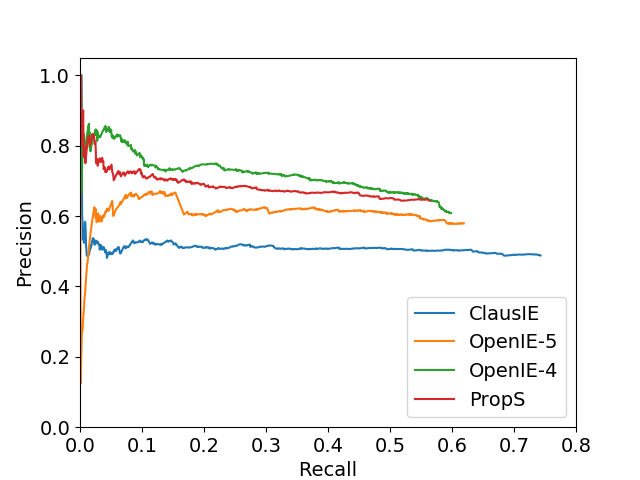
\includegraphics[width=0.7\columnwidth]{images/carb/oie16.png}
            \caption{Comparison of Open IE systems using OIE2016}
            \label{fig:pr_oie16}
        \end{figure}
        
        % PR_carb
        \begin{figure}[h!]
            \centering
        \vspace*{-3ex}
        %   \includegraphics[width=\linewidth]{carb.PNG}
            \includegraphics[width=0.7\columnwidth]{images/carb/carb.png}
            \caption{Evaluation of Open IE systems using CaRB}
            \label{fig:pr_carb}
        \end{figure}

    
    \subsection{Human Verification}
        Through human verification, our goal is to learn the accurate ranking for ClausIE and PropS.  We randomly select 100 test sentences and evaluate both system extractions on this subset. 

        We assess the correct ranking between PropS and ClausIE using MTurk. Four workers are shown the extractions from both systems in random order and asked to either choose one of the systems as the better one or indicate that both are equal. The majority opinion of these four is considered as the correct ranking for that sentence, an equal split leading to a tie. In this experiment, we only allow MTurk workers who have been trained for Open IE for the crowdsourcing task to participate.

        Of these 100 sentences, PropS is chosen to have performed better for 15, ClausIE for 69 whereas 16 ended up in a tie. ClausIE is indeed considered the better system in human evaluation, and we verify that CaRB gives an accurate ranking of these two systems compared to OIE2016. 

\section{Conclusion}
    We contribute CaRB \citep{bhardwaj&al19}, a crowdsourced dataset for evaluation and comparison of Open IE systems. We assess this dataset against an expert-annotated dataset and find that it is dramatically more accurate than the existing OIE2016 benchmark dataset. 

    We also implement a scorer that computes precision, recall and area under p-r curve for a given system output by matching it with the CaRB dataset. In designing our scorer, we make several design choices that deviate from prior work in both match scores and also in finding the best match for a tuple. We believe our scheme treats various systems fairly. And in one case where CaRB and OIE2016 give different rankings to two Open IE systems, we demonstrate via human evaluation that the ranking given by CaRB is the accurate one. We release the dataset and scorer for further use by research community. 



%%%%%%%%%%%%%%%%%%%%%%%%%%%%%%%%%%%%%%%%%%%%%%%%%%
% IMoJIE.

\chapter{IMoJIE - Iterative Memory Based Joint Open IE}
\label{chap:imojie}

\section{Overview}

    We design the first neural OpenIE system that uses sequential decoding of tuples conditioned on previous tuples. We achieve this by adding every generated extraction so far to the encoder. This iterative process stops when the \textit{EndOfExtractions} tag is generated by the decoder, allowing it to produce a variable number of extractions. We name our system \boldlongname\ (\boldshortname).

    CopyAttention uses a bootstrapping strategy, where the extractions from  OpenIE-4 \cite{christensen&al11,pal&al16} are used as training data. However, we believe that training on extractions of multiple systems is preferable. For example, OpenIE-4 benefits from high precision compared to ClausIE \cite{corro&al13}, which offers high recall. By aggregating extractions from both, \shortname{} could potentially obtain a better precision-recall balance.

    However, simply concatenating extractions from multiple systems does not work well, as it leads to redundancy as well as exaggerated noise in the dataset. 
    We devise an unsupervised \textbf{Score-and-Filter} mechanism to automatically select a subset of these extractions that are non-redundant and expected to be of high quality. Our approach scores all extractions with a scoring model, followed by filtering to reduce redundancy.

    We compare \shortname\ against several neural and non-neural systems, including our extension of CopyAttention that uses BERT \cite{devlin&al19} instead of an LSTM at encoding time, which forms a very strong baseline. On the recently proposed CaRB metric, which penalizes redundant extractions \cite{bhardwaj&al19}, \shortname\ outperforms CopyAttention by about 18 pts in F1 and our strong BERT baseline by 2 pts, establishing a new state of the art for OpenIE. We release \shortname\ \& all related resources for further research\footnote{\protect\url{https://github.com/dair-iitd/imojie}}.

\section{Sequencial Decoding Model}

    % Seq decoding model
    \begin{figure*}[h]
    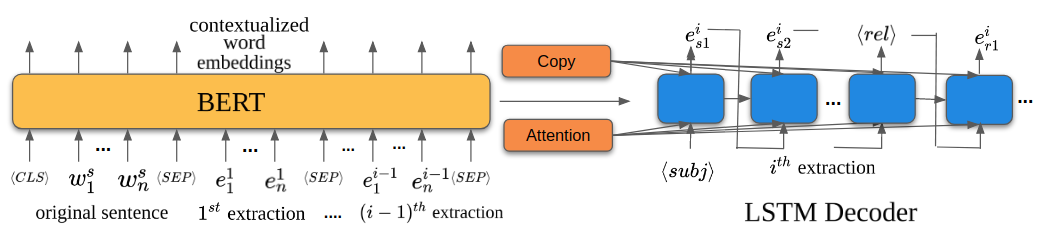
\includegraphics[width=.99\hsize]{images/imojie/model.png}
    \caption{One step of the sequential decoding process, for generating the $i^\text{th}$ extraction, which takes the original sentence and all extractions numbered $1,\ldots,i-1$, previously generated, as input.}
    \label{fig:seq_dec}
    \end{figure*}

    We now describe \shortname{}, our generative approach that can output a variable number of diverse extractions per sentence. The architecture of our model is illustrated in Figure \ref{fig:seq_dec}. At a high level, the next extraction from a sentence is best determined in context of all other tuples extracted from it so far.  Hence, \shortname{} uses a decoding strategy that generates extractions in a sequential fashion, one after another, each one being aware of all the ones generated prior to it.

    This kind of sequential decoding is made possible by the use of an \textit{iterative memory}. Each of the generated extractions are added to the memory so that the next iteration of decoding has access to all of the previous extractions. We simulate this iterative memory with the help of BERT encoder, whose input includes the [\textit{CLS}] token and original sentence appended with the decoded extractions so far, punctuated by the separator token [\textit{SEP}] before each extraction.

    \shortname{} uses an LSTM  decoder, which is initialized with the embedding of [\textit{CLS}] token. The contextualized-embeddings of all the word tokens are used for the Copy \citep{gu&al16} and Attention \citep{bahdanau&al15} modules. The decoder generates the tuple one word at a time, producing $\langle \textit{rel} \rangle$ and $\langle \textit{obj} \rangle$ tokens to indicate the start of relation and object respectively. The iterative process continues until the \textit{EndOfExtractions} token is generated.

    The overall process can be summarized as:
    \begin{enumerate}
        \item Pass the sentence through the Seq2Seq architecture to generate the first extraction.
        \item Concatenate the generated extraction with the existing input and pass it again through the Seq2Seq architecture to generate the next extraction.
        \item Repeat Step 2 until the \textit{EndOfExtractions} token is generated.
    \end{enumerate}

    \shortname{} is trained using a cross-entropy loss between the generated output and the gold output.


\section{Aggregating Bootstrapped Data}
    
    \subsection{Single Bootstrapping System}

        To train generative neural models for the task of OpenIE, we need a set of sentence-extraction pairs. It is ideal to curate such a training dataset via human annotation, but that is impractical, considering the scale of training data required for a neural model. We follow \citet{cui&al18}, and use  bootstrapping --- using extractions from a pre-existing OpenIE system as `silver'-labeled (as distinct from `gold'-labeled) instances to train the neural model. We first order all extractions in the decreasing order of confidences output by the original system. We then construct training data in \shortname's input-output format, assuming that this is the order in which it should produce its extractions.

    \subsection{Multiple Bootstrapping Systems}

        % score-and-filter
        \begin{figure*}[h]
            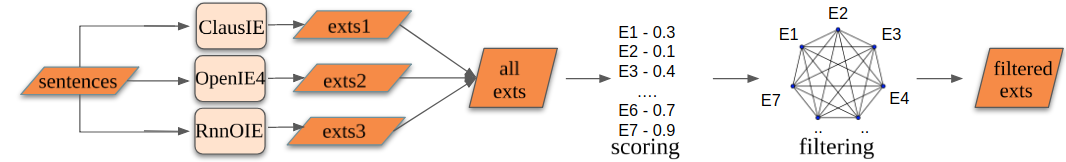
\includegraphics[width=.99\hsize]{images/imojie/score_filter.png}
            \caption{Ranking-Filtering subsystem for combining extractions from multiple open IE systems in an unsupervised fashion.  (`Exts'=extractions.)}
            \label{fig:score_filter}
        \end{figure*}

        Different OpenIE systems have diverse quality characteristics. For example, the human-estimated (precision, recall) of OpenIE-4 is $(\textbf{61},43)$ while that of ClausIE is $(40,\textbf{50})$. Thus, by using their combined extractions as the bootstrapping dataset, we might potentially benefit from the high precision of OpenIE-4 and high recall of ClausIE.

        However, simply pooling all extractions would not work, because of the following serious hurdles.
        \begin{description}
        \item[No calibration:] Confidence scores assigned by different systems are not calibrated to a comparable scale.
        \item[Redundant extractions:] Beyond exact duplicates, multiple systems produce similar extractions with low marginal utility.
        \item[Wrong extractions:] Pooling inevitably pollutes the silver data and can amplify incorrect instances, forcing the downstream open IE system to learn poor-quality extractions.
        \end{description}
        We solve these problems using a \textbf{Score-and-Filter} framework, shown in Figure~\ref{fig:score_filter}.

        \vspace{0.5ex}
        \noindent \textbf{Scoring:}
        All systems are applied on a given sentence, and the pooled set of extractions are scored such that good (correct, informative) extractions generally achieve higher values compared to bad (incorrect) and redundant ones.  In principle, this score may be estimated by the generation score from \shortname, trained on a single system. 
        
        In practice, such a system is likely to consider extractions similar to its bootstrapping training data as good, while disregarding extractions of other systems, even though those extractions may also be of high quality. 
        To mitigate this bias, we use an \shortname{} model, pre-trained on a \textit{random bootstrapping dataset}. The random bootstrapping dataset is generated by picking extractions for each sentence randomly from any one of the bootstrapping systems being aggregated. We assign a score to each extraction in the pool based on the confidence value given to it by this \shortname~(Random) model.

        \vspace{0.5ex}
        \noindent \textbf{Filtering:}
        We now filter this set of extractions for redundancy. 
        Given the set of ranked extractions in the pool, we wish to select that subset of extractions that have the best confidence scores (assigned by the random-boostrap model), while having minimum similarity to the other selected extractions.

        We model this goal as the selection of an optimal subgraph from a suitably designed complete weighted graph. Each node in the graph corresponds to one extraction in the pool. Every pair of nodes $(u,v)$ are connected by an edge. Every edge has an associated weight $R(u,v)$ signifying the similarity between the two corresponding extractions. Each node $u$ is assigned a score $f(u)$ equal to the confidence given by the random-bootstrap model.

        Given this graph $G = (V, E)$ of all pooled extractions of a sentence, we aim at selecting a subgraph $G' = (V', E')$ with $V' \subseteq V$, such that the most significant ones are selected, whereas the extractions redundant with respect to already-selected ones are discarded. Our objective is
        \begin{equation} \label{eq:1}
        \max_{G'\subseteq G} \sum_{i=1}^{|V'|} f(u_i) -
        \sum_{j=1}^{|V'|-1}\sum_{k=j+1}^{|V'|} R(u_{j},u_{k}),
        \end{equation}
        where $u_{i}$ represents node $i\in V'$.  
        %Here, $f(u_{i})$ represents node score for vertex $u_{i}$, i.e., the score for each triple obtained using the random-bootstrap model. 
        We compute $R(u,v)$ as the ROUGE2 score between the serialized triples represented by nodes $u$ and $v$. We can intuitively understand the first term as the aggregated sum of significance of all selected triples and second term as the redundancy among these triples.

        If $G$ has $n$ nodes, we can pose the above objective as:
        \begin{align}
        \max_{\bm{x} \in \{0,1\}^{n}}  \bm{x}^\top \bm{f} - \bm{x}^\top \bm{R} \bm{x},
        \end{align}
        where $\bm{f} \in \mathbb{R}^n$ representing the node scores, i.e., $f[i]=f(u_{i})$, and
        $\bm{R} \in \mathbb{R}^{n\times n}$ is a symmetric matrix with entries $R_{j,k}=\text{ROUGE2}(u_{j},u_{k})$.
        $\bm{x}$ is the decision vector, with $x[i]$ indicating whether a particular node $u_i \in V'$ or not. This is an instance of Quadratic Boolean Programming and is NP-hard, but in our application $n$ is modest enough that this is not a concern.  We use the QPBO (Quadratic Pseudo Boolean Optimizer) solver\footnote{\href{https://pypi.org/project/thinqpbo/}{https://pypi.org/project/thinqpbo/}} \cite{Rother2007OptimizingBM} to find the optimal $\bm{x}^*$ and recover~$V'$.

\section{Experimental Setup}
    \subsection{Training Data Construction}

        %To train a seq2seq model, we require a large training corpus of labeled data. 
        We obtain our training sentences by scraping Wikipedia, because Wikipedia is a comprehensive source of informative text from diverse domains, rich in entities and relations.  
        Using sentences from Wikipedia ensures that our model is not biased towards data from any single domain.

        We run OpenIE-4\footnote{\href{https://github.com/knowitall/openie}{https://github.com/knowitall/openie}}, ClausIE\footnote{\href{https://www.mpi-inf.mpg.de/departments/databases-and-information-systems/software/clausie}{https://www.mpi-inf.mpg.de/clausie}} and RnnOIE\footnote{\href{https://github.com/gabrielStanovsky/supervised-oie}{https://github.com/gabrielStanovsky/supervised-oie}} on these sentences to generate a set of OpenIE tuples for every sentence, which are then ranked and filtered using our Score-and-Filter technique. 
        These tuples are further processed to generate training instances in \shortname's input-output format. 

        Each sentence contributes to multiple (input, output) pairs for the \shortname{} model. The first training instance contains the sentence itself as input and the first tuple as output. For example, (``I ate an apple and an orange.'', ``I; ate; an apple''). The next training instance, contains the sentence concatenated with previous tuple as input and the next tuple as output (``I ate an apple and an orange. [SEP] I; ate; an apple'',  ``I; ate; an orange''). The final training instance generated from this sentence includes all the extractions appended to the sentence as input and \textit{EndOfExtractions} token as the output. Every sentence gives the seq2seq learner one training instance more than the number of tuples. 

        While forming these training instances, the tuples are considered in decreasing order of their confidence scores.  If some OpenIE system does not provide confidence scores for extracted tuples, then the output order of the tuples may be used.  

    \subsection{Dataset and Evaluation Metrics}

        We use the CaRB data and evaluation framework \cite{bhardwaj&al19} to evaluate the systems\footnote{Our reported CaRB scores for OpenIE-4 and OpenIE-5 are slightly different from those reported by \citet{bhardwaj&al19}. The authors of CaRB have verified our values.} at different confidence thresholds, yielding a precision-recall curve. We identify three important summary metrics from the P-R curve. 

        \todo{resolve diff in scores in carb and imojie paper, remove footnote}

        \noindent \textbf{Optimal F1}: We find the point in the P-R curve corresponding to the largest F1 value and report that.  This is the operating point for getting extractions with the best precision-recall trade-off.

        \noindent \textbf{AUC}: This is the area under the P-R curve. This metric is useful when the downstream application can use the confidence value of the extraction.

        \noindent \textbf{Last F1}: This is the F1 score computed at the point of zero confidence. This is of importance when we cannot compute the optimal threshold, due to lack of any gold-extractions for the domain. Many downstream applications of OpenIE, such as text comprehension \citep{stanovsky&al15} and sentence similarity estimation \citep{janara&al14}, use \emph{all} the extractions output by the OpenIE system. Last~F1 is an important measure for such applications.

    \subsection{Comparison Systems}
        % TABLE - SCORES TABLE
        \begin{table}[h]
            \centering {\footnotesize
            \begin{tabular}{lccc}
            \hline
            \textbf{System} & \multicolumn{3}{c}{\textbf{Metric}}  \\
            & \multicolumn{1}{c}{Opt. F1} & \multicolumn{1}{c}{AUC} & \multicolumn{1}{c}{Last F1}\\
            \hline
            Stanford-IE & 23 & 13.4 & 22.9 \\
            OllIE & 41.1 & 22.5 & 40.9 \\ 
            PropS & 31.9 & 12.6 & 31.8 \\ 
            MinIE & 41.9 & -$^*$ & 41.9 \\ 
            OpenIE-4 & 51.6 & 29.5 & 51.5 \\ 
            OpenIE-5 & 48.5 & 25.7 & 48.5 \\ 
            ClausIE & 45.1 & 22.4 & 45.1 \\ \hline 
            CopyAttention & 35.4 & 20.4 & 32.8 \\ 
            RNN-OIE & 49.2 & 26.5 & 49.2 \\ 
            Sense-OIE & 17.2 & -$^*$ & 17.2 \\ 
            Span-OIE & 47.9 & -$^*$ & 47.9 \\
            CopyAttention + BERT & 51.6 & 32.8 & 49.6 \\ \hline
            % \shortname~(OpenIE-4) & 53.1 & \textbf{33.5} & 52.6 \\ 
            \shortname~ & \textbf{53.5} & \textbf{33.3} & \textbf{53.3} \\ \hline
            \end{tabular} }
            \caption{Comparison of various OpenIE systems - non-neural, neural and proposed models. (*)~Cannot compute AUC as Sense-OIE, MinIE do not emit confidence values for extractions and released code for Span-OIE does not provision calculation of confidence values. In these cases, we report the Last F1 as the Opt. F1}
            % as system does not give confidence values for extractions.}
            \label{tab:scores-table}
        \end{table}    
    
        We compare \shortname{} against several non-neural baselines, including Stanford-IE, OpenIE-4, OpenIE-5, ClausIE, PropS, MinIE, and OLLIE. We also compare against the sequence labeling baselines of RnnOIE, SenseOIE, and the span selection baseline of SpanOIE. Probably the most closely related baseline to us is the neural generation baseline of CopyAttention. To increase CopyAttention's diversity, we compare against an English version of Logician, which adds coverage attention to a single-decoder model that emits all extractions one after another. We also compare against CopyAttention augmented with diverse beam search \cite{diversebeam} --- it adds a diversity term to the loss function so that new beams have smaller redundancy with respect to all previous beams.

        Finally, because our model is based on BERT, we reimplement CopyAttention with a BERT encoder --- this forms a very strong baseline for our task. Table \ref{tab:scores-table} enlists the CaRB scores of these systems.

    \subsection{Implementation}

        We implement \shortname{} in the AllenNLP framework\footnote{\href{https://github.com/allenai/allennlp}{https://github.com/allenai/allennlp}} \citep{gardner2018allennlp} using Pytorch~1.2.  We use ``BERT-small'' model for faster training. Other hyper-parameters include learning rate for BERT, set to $2\times10^{-5}$, and learning rate, hidden dimension, and word embedding dimension of the decoder LSTM, set to $(10^{-3}, 256, 100)$, respectively.

        Since the model or code of CopyAttention \citep{cui&al18} were not available, we implemented it ourselves. Our implementation closely matches their reported scores, achieving (F1, AUC) of (56.4, 47.7) on the OIE2016 benchmark.

\section{Results and Analysis}

    \subsection{Performance of Existing Systems}

        \emph{How well do the neural systems perform as compared to the rule-based systems?}

        Using CaRB evaluation, we find that, contrary to previous papers, neural OpenIE systems are not necessarily better than prior non-neural systems (Table~\ref{tab:scores-table}).  Among the systems under consideration, the best non-neural system reached Last~F1 of 51.5, whereas the best existing neural model could only reach~49.2. Deeper analysis reveals that CopyAttention produces redundant extractions conveying nearly the same information, which CaRB effectively penalizes.  RnnOIE performs much better, however suffers due to its lack of generating auxilliary verbs and implied prepositions. Example, it can only generate (Trump; President; US) instead of (Trump; is President of; US) from the sentence ``US President Trump...". Moreover, it is trained only on limited number of pseudo-gold extractions, generated by \citet{michael&al18}, which does not take advantage of boostrapping techniques.


        \vspace{0.5ex}
    \subsection{Performance of \shortname}
        \emph{How does \shortname{} perform compared to the previous neural and rule-based systems?} 
        % \noindent{\bfseries Performance of \shortname:}  

        % TABLE - IMOJIE vs OpenIE-4 Example
        \begin{table*}[h]
            \centering
            {\small
            \resizebox{\textwidth}{!}{%
            \begin{tabular}{|c|l|}
            \hline
            \textbf{Sentence} & \begin{tabular}[c]{@{}l@{}}Greek and Roman pagans , who saw their relations with the gods in political and social\\  terms , scorned the man who constantly trembled with fear at the thought of the gods ,\\  as a slave might fear a cruel and capricious master .\end{tabular} \\ \hline
            \textbf{OpenIE-4} & ( the man ;  constantly trembled ;   ) \\ \hline
            \textbf{\begin{tabular}[c]{@{}c@{}}IMOJIE\\ \end{tabular}} & \begin{tabular}[c]{@{}l@{}}( a slave ; might fear ; a cruel and capricious master )\\ ( Greek and Roman pagans ; scorned ; the man who ... capricious master )\\ ( the man ; constantly trembled ; with fear at the thought of the gods )\\ ( Greek and Roman pagans ; saw ; their relations with the gods in political and social terms )\end{tabular} \\ \hline
            \end{tabular}}
            }
            \caption{\shortname~ vs. OpenIE-4. Pipeline nature of OpenIE-4 can get confused by long convoluted sentences, but \shortname{} responds gracefully.}
            \label{tab:quality-example}
        \end{table*}

        In comparison with existing neural and non-neural systems, \shortname{} trained on aggregated bootstrapped data performs the best.  It outperforms OpenIE-4, the best existing OpenIE system, by 1.9 F1 pts, 3.8 pts of AUC, and 1.8 pts of Last-F1. Qualitatively, we find that it makes fewer mistakes than OpenIE-4, probably because OpenIE-4 accumulates errors from upstream parsing modules (see Table \ref{tab:quality-example}). 

        % TABLE - REDUNDANCY EXAMPLE (IMoJIE vs Copy Attention)
        \begin{table*}[h]
            \centering
            {\small
            \resizebox{\textwidth}{!}{%
            \begin{tabular}{|c|l|}
            \hline
            \textbf{Sentence} & \begin{tabular}[c]{@{}l@{}}He was appointed Commander of the Order of the British Empire in the 1948\\  Queen's Birthday Honours and was knighted in the 1953 Coronation Honours .\end{tabular} \\ \hline
            \textbf{CopyAttention} & \begin{tabular}[c]{@{}l@{}}( He ; was appointed ; Commander ... Birthday Honours )\\( He ; was appointed ; Commander ... Birthday Honours and was knighted ... Honours )\\( Queen 's Birthday Honours ; was knighted ; in the 1953 Coronation Honours )\\( He ; was appointed ; Commander of the Order of the British Empire in the 1948 )\\( the 1948 ; was knighted ; in the 1953 Coronation Honours)\end{tabular} \\ \hline
            \textbf{\begin{tabular}[c]{@{}l@{}}IMOJIE\\ \end{tabular}} & \begin{tabular}[c]{@{}l@{}}( He ; was appointed ; Commander of the Order ... Birthday Honours )\\( He ; was knighted ; in the 1953 Coronation Honours )\end{tabular} \\ \hline
            \end{tabular}}
            }
            \caption{\shortname~ vs. CopyAttention. CopyAttention suffers from stuttering, which \shortname{} does not.}
            \label{tab:redundancy-example}
        \end{table*}

        \shortname{} outperforms CopyAttention by large margins -- about 18 Optimal F1 pts and 13 AUC pts. Qualitatively, it outputs non-redundant extractions through the use of its iterative memory (see Table~\ref{tab:redundancy-example}), and a variable number of extractions owing to the \textit{EndofExtractions} token.
        It also outperforms CopyAttention with BERT, which is a very strong baseline, by 1.9 Opt. F1 pts, 0.5 AUC and 3.7 Last F1 pts. \shortname{} consistently outperforms CopyAttention with BERT over different bootstrapping datasets (see Table~\ref{tab:bootstrapping-datasets}).

        \begin{figure}[t]
            \centering
        \vspace*{-3ex}
        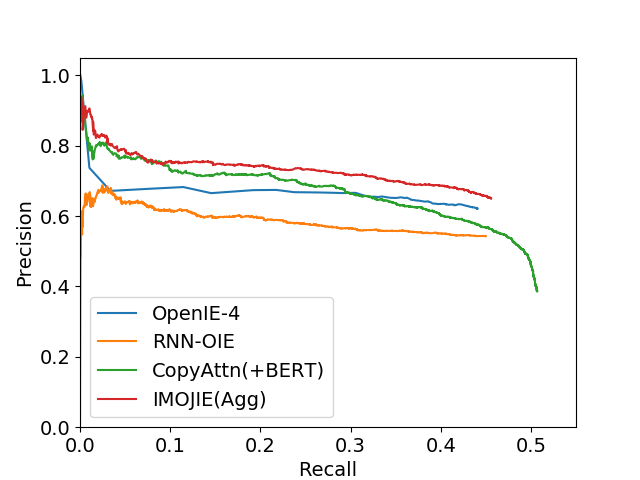
\includegraphics[scale=0.80]{images/imojie/imojie.png}
        \caption{Precision-Recall curve of OpenIE Systems.}
        \label{fig:pr-curve}
        \end{figure}

        Figure~\ref{fig:pr-curve} shows that the precision-recall curve of \shortname{} is consistently above that of existing OpenIE systems, emphasizing that \shortname{} is consistently better than them across the different confidence thresholds. We do find that CopyAttention+BERT outputs slightly higher recall at a significant loss of precision (due to its beam search with constant size), which gives it some benefit in the overall AUC. CaRB evaluation of SpanOIE\footnote{\href{https://github.com/zhanjunlang/Span\_OIE}{https://github.com/zhanjunlang/Span\_OIE}} results in (precision, recall, F1) of (58.9, 40.3, 47.9). SpanOIE sources its training data only from OpenIE-4. In order to be fair, we compare it against \shortname{} trained only on data from OpenIE-4 which evaluates to (60.4, 46.3, 52.4). Hence, \shortname{} outperforms SpanOIE, both in precision and recall.

        Attention is typically used to make the model focus on words which are considered important for the task. But the \shortname{} model successfully uses attention to \emph{forget} certain words, those which are already covered. 
        
        Consider, the sentence ``He served as the first prime minister of Australia and became a founding justice of the High Court of Australia''. 
        Given the previous extraction (He; served; as the first prime minister of Australia), the BERT’s attention layers figure out that the words `prime' and `minister' have already been covered, and thus push the decoder to prioritize `founding' and `justice'.
        Appendix~\ref{sec:visualize_attention} analyzes the attention patterns of the model when generating the intermediate extraction in the above example and shows that \shortname{} gives less attention to already covered words.

        \vspace{0.5ex}
    \subsection{Redundancy}
        \emph{What is the extent of redundancy in \shortname{} when compared to earlier OpenIE systems?}

        % TABLE - REDUNDANCY REMOVAL EXPERIMENT
        \begin{table}[h]
            \centering {\footnotesize
            \begin{tabular}{lccc}
            \hline
            \textbf{System} & \multicolumn{3}{c}{\textbf{Metric}}  \\
            & \multicolumn{1}{c}{Opt. F1} & \multicolumn{1}{c}{AUC} & \multicolumn{1}{c}{Last F1}\\
            \hline
            CopyAttention & 35.4 & 20.4 & 32.8 \\ 
            CoverageAttention & 41.8 & 22.1 & 41.8 \\ 
            CoverageAttention+BERT & 47.9 & 27.9 & 47.9 \\ 
            Diverse Beam Search & 46.1 & 26.1 & 39.6 \\ 
            \shortname~ (w/o BERT) & 37.9 & 19.1 & 36.6 \\ 
            \shortname~ & \textbf{53.2} & \textbf{33.1} & \textbf{52.4} \\ \hline
            \end{tabular} }
            \caption{Models to solve the redundancy issue prevalent in Generative Neural OpenIE systems. All systems are bootstrapped on OpenIE-4.}
            \label{tab:redundancy_rem_exp}
        \end{table}

        We also investigate other approaches to reduce redundancy in CopyAttention, such as Logician's coverage attention (with both an LSTM and a BERT encoder) as well as diverse beam search. 
        Table~\ref{tab:redundancy_rem_exp} reports that both these approaches indeed make significant improvements on top of CopyAttention scores. 
        In particular, qualitative analysis of diverse beam search output reveals that the model gives out different words in different tuples in an effort to be diverse, without considering their correctness. 
        Moreover, since this model uses beam search, it still outputs a fixed number of tuples.

        % TABLE - BOOTSTRAPPING DATASETS
        \begin{table*}
        \centering {\footnotesize
        \begin{tabular}{lcccc}
        \hline
        \textbf{System} & \multicolumn{4}{c}{\textbf{Bootstrapping System}}  \\
        & \multicolumn{1}{c}{OpenIE-4} & \multicolumn{1}{c}{OpenIE-5} & \multicolumn{1}{c}{ClausIE} & \multicolumn{1}{c}{RnnOIE}\\
        \hline
        Base & 50.7, 29, 50.7 & 47.4, 25.1, 47.4 & 45.1, 22.4, 45.1 & 49.2, 26.5, 49.2 \\ 
        CopyAttention+BERT & 51.6, 32.8, 49.6 & 48.7, \textbf{29.4}, 48.0 & 47.4, 30.2, 43.6 & 47.9, 30.6, 41.1 \\ 
        \shortname & \textbf{53.2}, \textbf{33.1}, \textbf{52.4} & \textbf{48.8}, 27.9, \textbf{48.7} & \textbf{49.2}, \textbf{31.4}, \textbf{45.5} & \textbf{51.3}, \textbf{31.1}, \textbf{50.8} \\ \hline
        \end{tabular} }
        \caption{Evaluating models trained with different bootstrapping systems.}
        \label{tab:bootstrapping-datasets}
        \end{table*}

        This analysis naturally suggested the \shortname~(w/o BERT) model --- an \shortname{} variation that uses an LSTM encoder instead of BERT. Unfortunately, \shortname~(w/o BERT) is behind the CopyAttention baseline by 12.1 pts in AUC and 4.4 pts in Last~F1. We hypothesize that this is because the LSTM encoder is unable to learn how to capture \textit{inter-fact dependencies} adequately --- the input sequences are too long for effectively training LSTMs.

        This explains our use of Transformers (BERT) instead of the LSTM encoder to obtain the final form of \shortname.  With a better encoder, \shortname{} is able to perform up to its potential, giving an improvement of \textbf{(17.8, 12.7, 19.6)} pts in (Optimal~F1, AUC, Last~F1) over existing seq2seq OpenIE systems.

        We further measure two quantifiable metrics of redundancy:
        \begin{description}
        \item[Mean Number of Occurrences (MNO):] The average number of tuples, every output word appears in.
        \item[Intersection Over Union (IOU):] Cardinality of intersection over cardinality of union of words in the two tuples, averaged over all pairs of tuples.
        \end{description}

        These measures were calculated after removing stop words from tuples.  Higher value of these measures suggest higher redundancy among the extractions.  \shortname{} is significantly better than CopyAttention+BERT, the strongest baseline, on both these measures (Table~\ref{tab:RED}). Interestingly, \shortname{} has a lower redundancy than even the gold triples; this is due to imperfect recall.


        % TABLE - REDUNDANCY Experiments
        \begin{table}[h]
            \centering {\footnotesize
            \begin{tabular}{lccc}
            \hline
            \textbf{Extractions} & \multicolumn{3}{c}{\textbf{Metric}}  \\
            & \multicolumn{1}{c}{MNO} & \multicolumn{1}{c}{IOU} & \multicolumn{1}{c}{\#Tuples}\\
            \hline
            CopyAttention+BERT &  2.805 & 0.463 & 3159 \\ 
            \textbf{IMOJIE} & \textbf{1.282} & \textbf{0.208} & \textbf{1620} \\ 
            Gold & 1.927 & 0.31 & 2650 \\ \hline
            \end{tabular} }
            \caption{Measuring redundancy of extractions. MNO stands for Mean Number of Occurrences. IOU stands for Intersection over Union.}
            \label{tab:RED}
        \end{table}

        \vspace{0.5ex}
    \subsection{The Value of Iterative Memory}

        \emph{To what extent does the \shortname~style of generating tuples improve performance, over and above the use of BERT?} 

        We add BERT to CopyAttention model to generate another baseline for a fair comparison against the \shortname{} model. When trained only on OpenIE-4, \shortname{} continues to outperform CopyAttention+BERT baseline by (1.6, 0.3, 2.8) pts in (Optimal~F1, AUC, Last~F1), which provides strong evidence that the improvements are not solely by virtue of using a better encoder.
        We repeat this experiment over different (single) bootstrapping datasets. Table \ref{tab:bootstrapping-datasets} depicts that \shortname~consistently outperforms CopyAttention+BERT model.

        We also note that the order in which the extractions are presented to the model (during training) is indeed important. On training IMoJIE using a randomized-order of extractions, we find a decrease of 1.6 pts in AUC (averaged over 3 runs).

        % \vspace{0.5ex}
        % \noindent\textbf{Ablation Study over Bootstrapping Datasets:} We now assess the value of bootstrapping from multiple extraction systems. The ablation study over the datasets (Table \ref{tab:dataset-ablation}) suggests that the model trained on all three aggregated datasets perform better than models trained on either of the single/doubly-aggregated datasets.
        \vspace{0.5ex}
    \subsection{The value of Score-and-Filter}
        % \noindent\textbf{The Value of Score-and-Filter:} 
        \emph{To what extent does the scoring and filtering approach lead to improvement in performance?} 

        \shortname{} aggregates extractions from multiple systems through the scoring and filtering approach. It uses extractions from OpenIE-4 (190K), ClausIE (202K) and RnnOIE (230K) to generate a set of 215K tuples. Table \ref{tab:dataset-aggregation1} reports that \shortname{} does not perform well when this aggregation mechanism is turned off. We also try two supervised approaches to aggregation, by utilizing the gold extractions from CaRB's dev set.
        
        \begin{table}[h]
            \centering {\footnotesize
            \begin{tabular}{lccc}
            \hline
            \textbf{Filtering} & \multicolumn{3}{c}{\textbf{Metric}}  \\
            & \multicolumn{1}{c}{Opt. F1} & \multicolumn{1}{c}{AUC} & \multicolumn{1}{c}{Last F1}\\
            \hline
            None & 49.7 & \textbf{34.5} & 37.4 \\ 
            Extraction-based & 46 & 29.2 & 44.9 \\ 
            Sentence-based &  49.5 & 32.7 & 48.6\\ 
            Score-And-Filter & \textbf{53.5} & 33.3 & \textbf{53.3} \\ \hline
            \end{tabular} }
            \caption{Performance of \shortname{} on aggregated dataset \textbf{OpenIE-4+ClausIE+RnnOIE}, with different filtering techniques. For comparison, SenseOIE trained on multiple system extractions gives an F1 of 17.2 on CaRB.}
            \label{tab:dataset-aggregation1}
        \end{table}

        \begin{itemize}
            \item \textbf{Extraction Filtering}: For every sentence-tuple pair, we use a binary classifier that decides whether or not to consider that extraction. The input features of the classifier are the \textit{[CLS]}-embeddings generated from BERT after processing the concatenated sentence and extraction. The classifier is trained over tuples from CaRB's dev set.
            \item \textbf{Sentence Filtering}: We use an \shortname{} model (bootstrapped over OpenIE-4), to score all the tuples. Then, a Multilayer Perceptron (MLP) predicts a confidence threshold to perform the filtering. Only extractions with scores greater than this threshold will be considered. The input features of the MLP include the length of sentence, \shortname~ (OpenIE-4) scores, and GPT \cite{Radford2018-GPT} scores of each extraction. This MLP is trained over sentences from CaRB's dev set and the gold optimal confidence threshold calculated by CaRB. 
        \end{itemize}
        We observe that the Extraction, Sentence Filtering are better than no filtering by by 7.5, 11.2 pts in Last F1, but worse at Opt. F1 and AUC. We hypothesise that this is because the training data for the MLP (640 sentences in CaRB's dev set), is not sufficient and the features given to it are not sufficiently discriminative.
        Thereby, we see the value of our unsupervised Score-and-Filter that improves the performance of \shortname{} by (3.8, 15.9) pts in (Optimal F1, Last F1). The 1.2 pt decrease in AUC is due to the fact that the \shortname{} (no filtering) produces many low-precision extractions, that inflates the AUC.


        % TABLE - DATASET ABLATION
        \begin{table}[h]
            \centering {\footnotesize
            \begin{tabular}{lccc}
            \hline
            \textbf{Bootstrapping } & \multicolumn{3}{c}{\textbf{Metric}}  \\
            \textbf{Systems} & \multicolumn{1}{c}{Opt. F1} & \multicolumn{1}{c}{AUC} & \multicolumn{1}{c}{Last F1} \\
            \hline
            ClausIE & 49.2 & 31.4 & 45.5 \\
            RnnOIE & 51.3 & 31.1 & 50.8 \\
            OpenIE-4 & 53.2 & 33.1 & 52.4 \\
            OpenIE-4+ClausIE & 51.5 & 32.5 & 47.1 \\ 
            OpenIE-4+RnnOIE & 53.1 & 32.1 & 53.0 \\ 
            ClausIE+RnnOIE & 50.9 & 32.2 & 49.8 \\ 
            All & \textbf{53.5} & \textbf{33.3} & \textbf{53.3} \\ \hline
            \end{tabular} }
            \caption{\shortname{} trained with different combinations of bootstrapping data from 3 systems - OpenIE-4, ClausIE, RNNOIE. Graph filtering is not used over single datasets.}
            \label{tab:dataset-ablation}
        \end{table}

        Table \ref{tab:dataset-ablation} suggests that the model trained on all three aggregated datasets perform better than models trained on any of the single/doubly-aggregated datasets. Directly applying the Score-and-Filter method on the test-extractions of RnnOIE+OpenIE-4+ClausIE gives (Optimal F1, AUC, Last F1) of (50.1, 32.4, 49.8). This shows that training the model on the aggregated dataset is important.

        \vspace{0.5ex}
        \noindent\textbf{Computational Cost}:
        The training times for CopyAttention+BERT, \shortname~ (OpenIE-4) and \shortname~ (including the time taken for Score-and-Filter) are 5 hrs, 13 hrs and 30 hrs respectively. This shows that the performance improvements come with an increased computational cost, and we leave it to future work to improve the computational efficiency of these models.


\section{Error Analysis}
    We randomly selected 50 sentences from the CaRB validation set. We consider only sentences where at least one of its extractions shows the error. We identified four major phenomena contributing to errors in the \shortname{} model: \newline
    (1) \textbf{Missing information:} 66\% of the sentences have at least one of the relations or arguments or both missing in predicted extractions, which are present in gold extractions. This leads to incomplete information. \newline
    (2) \textbf{Incorrect demarcation:} Extractions in 60\% of the sentences have the separator between relation and argument identified at the wrong place. \newline
    %For e.g., in sentence ``In October 2008 , Bond apologized to former U.S. Attorney ....", our system predicts (Bond; apologized; to former U.S. Attorney ....) whereas it should have been (Bond; apologized to; former U.S. Attorney ....). 
    (3) \textbf{Missing conjunction splitting:} In 32\% of the sentences, our system fails to separate out extractions by splitting a conjunction.  E.g., in the sentence ``US 258 and NC 122 parallel the river north \dots'', \shortname{} predicts just one extraction (US 258 and NC 122; parallel; \dots) as opposed to two separate extractions (US 258; parallel; \dots) and (NC 122; parallel; \dots) as in gold. \newline
    (4) \textbf{Grammatically incorrect extractions:} 38\% sentences have a grammatically incorrect extraction (when serialized into a sentence).  \newline
    Additionally, we observe 12\% sentences still suffering from \textbf{redundant} extractions and 4\% \textbf{miscellaneous} errors.

\section{Discussion}

    We propose \shortname~for the task of OpenIE. \shortname~significantly improves upon the existing OpenIE systems in all three metrics, Optimal F1, AUC, and Last F1, establishing a new State Of the Art system. Unlike existing neural OpenIE systems, \shortname~produces non-redundant as well as a variable number of OpenIE tuples depending on the sentence, by iteratively generating them conditioned on the previous tuples. Additionally, we also contribute a novel technique to combine multiple OpenIE datasets to create a high-quality dataset in a completely unsupervised manner. We release the training data, code, and the pretrained models.\footnote{\href{https://github.com/dair-iitd/imojie}{https://github.com/dair-iitd/imojie}}

    \shortname~ presents a novel way of using attention for text generation. \citet{bahdanau&al15} showed that attending over the input words is important for text generation. \citet{see&al17} showed that using a coverage loss to track the attention over the decoded words improves the quality of the generated output. We add to this narrative by showing that deep inter-attention between the input and the partially-decoded words (achieved by adding previous output in the input) creates a better representation for iterative generation of triples. This general observation may be of independent interest beyond OpenIE, such as in text summarization.

%%%%%%%%%%%%%%%%%%%%%%%%%%%%%%%%%%%%%%%%%%%%%%%%%%%%%%%%%%%%%%%%%%%%%%%%%%%%%%%%%%%%%%%%%%%%%%%%
% Uncategorised
%%%%%%%%%%%%%%%%%%%%%%%%%%%%%%%%%%%%%%%%%%%%%%%%%%%%%%%%%%%%%%%%%%%%%%%%%%%%%%%%%%%%%%%%%%%%%%%%




%%%%%%%%%%%%%%%%%%%%%%%%%%%%%%%%%%%%%%%%%%%%%%%%%%%%%%%%%%%%%%%%%%%%%%%%%%%%%%%%%%%%%%%%%%%%%%%%
% TABLES
%%%%%%%%%%%%%%%%%%%%%%%%%%%%%%%%%%%%%%%%%%%%%%%%%%%%%%%%%%%%%%%%%%%%%%%%%%%%%%%%%%%%%%%%%%%%%%%%
    


%%%%%%%%%%%%%%%%%%%%%%%%%%%%%%%%%%%%%%%%%%%%%%%%%%
% Remaining Problems.

\chapter{Remaining Problems}
\label{chap:remaining_problems}
\input{sections/06.problems_remaining.tex}

%%%%%%%%%%%%%%%%%%%%%%%%%%%%%%%%%%%%%%%%%%%%%%%%%%
% Conjunction Splitting.

\chapter{Conjunction Splitting}
\label{chap:conjunction_splitting}
\section{Problems Remaining in OpenIE}

    After addressing multiple key issues of OpenIE systems through \shortname, we sought to analyse the problems that are still prevalent with OpenIE systems. To begin with, we carefully analysed the erroneous outputs of \shortname\ and other systems. We could broadly categorise the remaining errors into the following types.

    \subsection{Missing Information}
        The major source of OpenIE errors is missing information in the OpenIE tuples. For \shortname, about 66\% of the sentences have at least one of the relations or arguments or both missing in predicted extractions, which are present in gold extractions. This leads to incomplete information. For eg.

        \begin{verbatim}
            Sentence:
            ``George got married to Alice in March beside the lake.''
            Set of Extractions with Missing Information:
            ( George ; got married ; )
            Gold Extractions:
            ( George ; got married to ; Alice )
            ( George ; got married in ; March )
            ( George ; got married beside ; the lake )
        \end{verbatim}

    \subsection{Incorrect Conjunction Splitting}

        One the guidelines of OpenIE is \emph{atomicity}. The principle of atomicity states that every tuple must be indivisible. In case of sentences with conjunctions, this translates to deriving multiple OpenIE tuples from the sentence, one with each conjunct. The output tuples where the coordination phrase has not been split are counted under the category of incorrect conjunction splitting. For eg.

        \begin{verbatim}
            Sentence:
            ``I ate an apple and an orange.''
            Incorrect Extraction:
            ( I ; ate ; an apple and an orange )
            Gold Extractions:
            ( I ; ate ; an apple )
            ( I ; ate ; an orange )
        \end{verbatim}
        
        It is worth noting that as much as 32\% of \shortname's errors are attributed to incorrect conjunction splitting.

    \subsection{Grammatical Errors}

        OpenIE tuples should not only identify the different parts of an extraction correctly, but should also lay them down in a grammatical structure. This means that when the extraction is serialised, the yielded sentence should be grammatical. For eg.

        \begin{verbatim}
            Sentence:
            ``US President Donald Trump''
            Incorrect Extraction:
            ( Donald Trump ; President ; US )
            Gold Extractions:
            ( Donald Trump ; is the president of ; US )
        \end{verbatim}

        Roughly 38\% of \shortname's errors were due to grammatical erros in its extractions.

    \subsection{Missing Output Context}

        OpenIE systems should be capable of generating the context of the output tuples whenever necessary. Rule-based systems like OpenIE-5 were able to generate context alongside the extractions yet \shortname\ and many recent OpenIE systems do not possess this ability. For eg.

        \begin{verbatim}
            Sentence:
            ``The police claimed, "Brutus broke into the house." ''
            Incorrect Extraction:
            ( Brutus ; broke into ; the house )
            Gold Extractions:
            [Context: The police claimed] ( Brutus ; broke into ; the house )
        \end{verbatim}

    \subsection{Coreference Resolution}

        OpenIE systems should be able to resolve coreferences in the sentence. They should generate each tuple such that the tuples do not depend on each other to clarify the their meaning. However, most OpenIE systems are not able to resolve coreferences till data. For eg.

        \begin{verbatim}
            Sentence:
            ``Alice ate an apple and then she went for a walk.''
            Incorrect Extraction:
            ( she ; went for ; a walk )
            Gold Extractions:
            ( Alice ; went for ; a walk )
        \end{verbatim}

    \subsection{Incorrect Identification of Boundaries}

        OpenIE systems are also known to incorrectly identify the relation and argument boundaries within a sentence. This includes errors like the object argument starts with a preposition instead of placing that preposition within the relation. In case of \shortname, nearly 60\% of the sentences have the separator between relation and argument identified at the wrong place. The major cause of this type of error is attributed to fallacies in the training data, however it may even creep in otherwise. For eg.

        \begin{verbatim}
            Sentence:
            ``Jonathon is going for a walk.''
            Incorrect Extraction:
            ( Jonathon ; is going ; for a walk )
            Gold Extractions:
            ( Jonathon ; is going for ; a walk )
        \end{verbatim}

\section{Why to Split Conjunctions?}

    OpenIE systems perform much better on short simple sentence as compared to long and complicated ones. This seems obvious since long sentences encompass multiple informations often intertwined in complex sentence structures. It requires much more expertise even for a human annotator to pick out all of them in the form of OpenIE tuples. However, when viewed in light of incorrect conjunction splitting done by OpenIE systems, this gives rise to a potent idea. We could design a separate module to explicitly break a complex sentence into several simple ones by splitting on conjunctions. Passing these simpler sentences through OpenIE systems inplace of the original sentence would yield higher quality extractions. This seemed to be a low-hanging fruit, hence we decided to go ahead with this idea.

    \subsection{Analysis of Existing Systems}
        In order to validate our hypothesis that a better module for conjunction splitting was actually required, we analysed the conjunction splitting ability of some popular rule-based systems. A separate analysis had shown that \verb|and| is the most frequent conjunction occuring in sentences with conjunctions. Hence, in order to expidite the current analysis, we chose only sentences with and. There were about 285 of them in the CaRB dev set. We manually annotated (refer table \ref{tab:conj_split_systems}) each of these sentences to determine how many of them were distributive i.e. how many sentences were such that they could be split into multiple simpler sentences.

        % TABLE: Conjunction Splitting Systems
        \begin{table*}[h]
            \centering
            \resizebox{0.5\textwidth}{!}{%
            \begin{tabular}{|c|c|c|c|}
            \hline
            \textbf{System} &
            \textbf{\begin{tabular}[c]{@{}c@{}}No. of\\ Sentences\\ with AND\end{tabular}} &
            \textbf{\begin{tabular}[c]{@{}c@{}}No. of\\ Distributive\\ Sentences\end{tabular}} &
            \textbf{\begin{tabular}[c]{@{}c@{}}Percentage of\\ Distributive\\ Sentences\end{tabular}} \\ \hline
            Gold     &     & 207 & 72.6 \\ \cline{1-1} \cline{3-4} 
            OpenIE-4 & 285 & 130 & 45.6 \\ \cline{1-1} \cline{3-4} 
            OpenIE-5 &     & 261 & 91.5 \\ \hline
            \end{tabular}%
            }
            \caption{Conjunction Splitting in Existing Rule-Based Systems}
            \label{tab:conj_split_systems}
        \end{table*}

        Of the 285 sentences annotated, 72.6\% were distributive. OpenIE-4 and OpenIE-5, two popular rule-based systems used for this analysis, split up 45.6\% and 91.5\% of these sentences respectively. This confirms that OpenIE-4 is too conservative in splitting conjunctions whereas OpenIE-5 is too aggressive. Moreover, none of them is close enough to the ideal split ratio of about 72\%. This analysis, therefore, confirms our hypothosis that a better module for conjunction splitting is required.

\section{HC-Tree Based Splitting}

    In this section, we discuss an approach for a conjunction-splitting model. The idea is based on \textbf{Hierarchical Coordination Trees}. An HC tree is an efficient representation of nested coordination phrases occuring in a sentence. Figure \ref{fig:hc_tree_eg} depicts an example of a complex sentence with nested coordination phrases and the corresponding HC tree.

    % HC Tree example
    \begin{figure*}[h]
        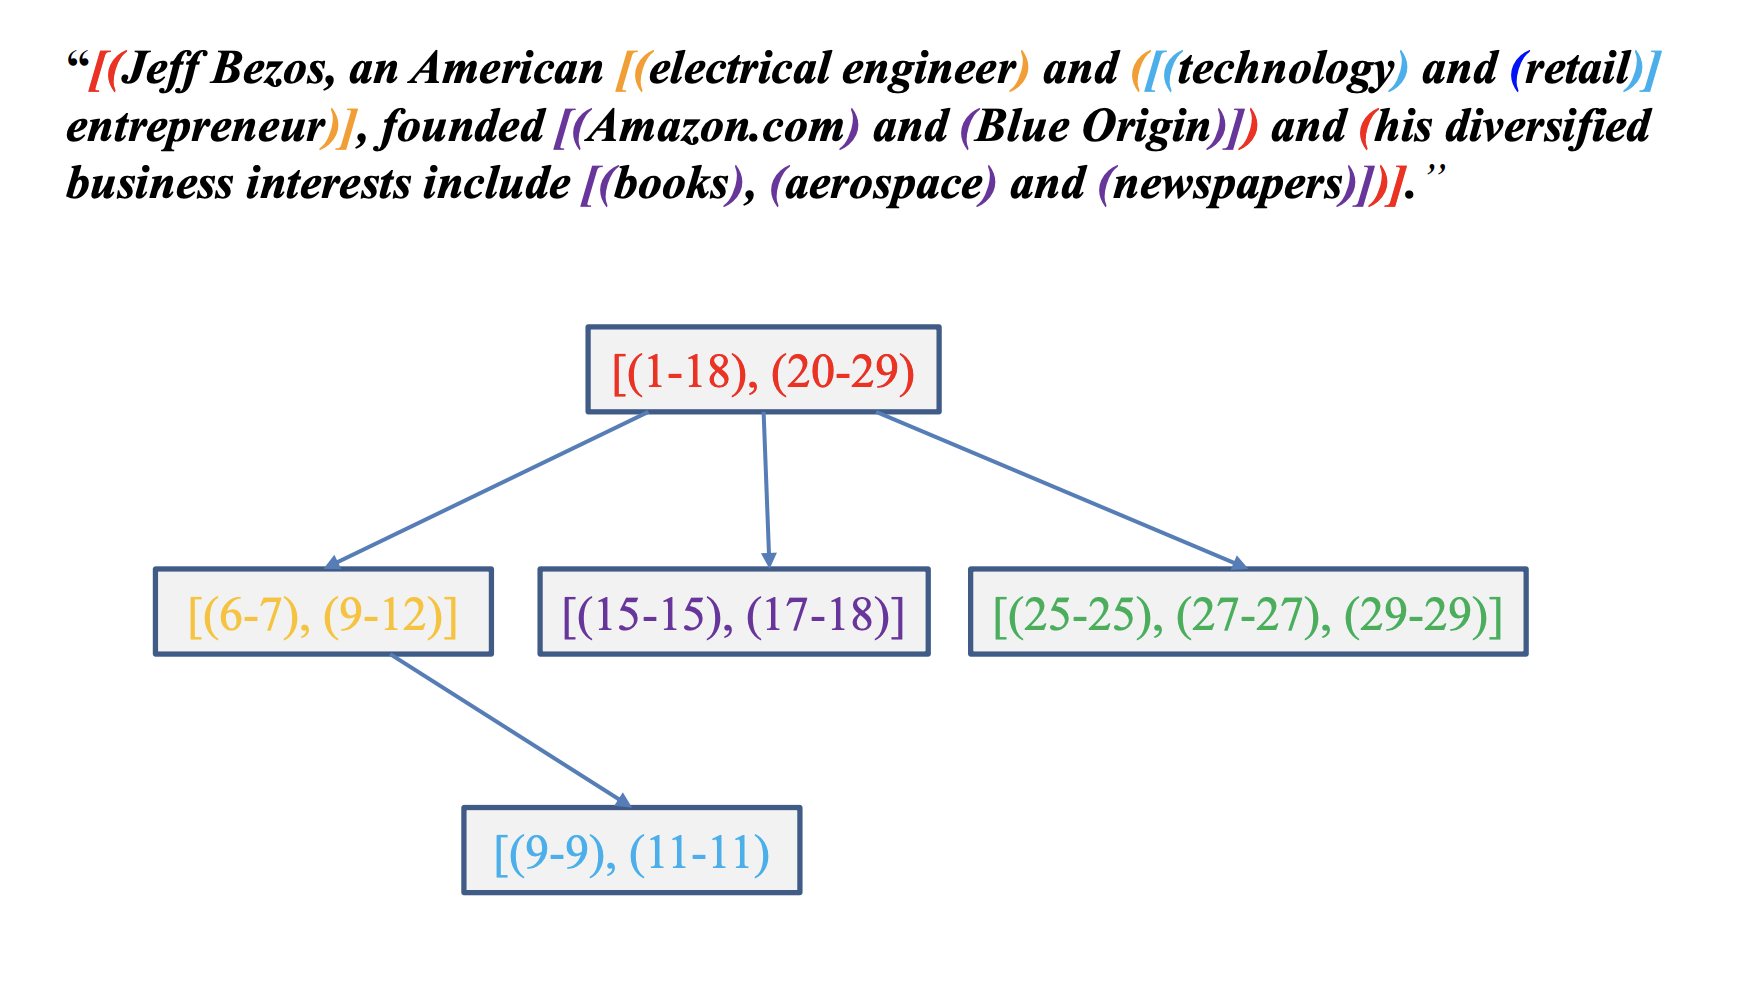
\includegraphics[width=.99\hsize]{images/hc_tree.png}
        \caption{Example of a sentence and its Hierarchical Coordination (HC) Tree}
        \label{fig:hc_tree_eg}
    \end{figure*}

    For our analysis, we use $[D_{i}]$ token at the beginning and end of each coordination phrase. Also, each conjunct is encapsulated with $[SS]$ and $[ES]$ tokens.

    \subsection{Properties of Conjuncts}
        It is important to discuss two key properties of conjuncts before diving into the approach. Consider the sentence \verb|I ate [D1] [SS] an apple [ES] and [SS] an orange [ES] [D1].| to understand the properties.
        \begin{enumerate}
            \item \textbf{Similarity:} The conjuncts are similar to each other in their syntactic form.
            
            For eg., \verb|an apple| and \verb|an orange| are syntactically similar.

            \item \textbf{Replaceability:} Each of the conjunct can potentially replace the entire coordination phrase in the original sentence and to yield a meaning sentence.
            
            For eg. \verb|``I ate an apple.''| and \verb|``I ate an orange.''| are both meaningful sentences.
            
        \end{enumerate}

    \subsection{Proposed Approach}

        \subsubsection{Step 1: Generation of HC Tree}
        
            First of all, we need to generate an HC tree for the given sentence. For this purpose, we use a sequence to sequence model with BERT as encoder and a Tree-Based decoder \citep{wang&al18}. We use data from PennTree Bank \citep{PennTreeBank} dataset due to the following reasons:
            \begin{enumerate}
                \item \textit{Sufficient number of sentences:} The PennTree Bank has a dev and test set of 1700 and 2416 sentences respectively.
                \item \textit{Contains coordinations upto depth 3:} PennTree Bank also has a significant number of sentences with coordinations nested at depths upto 3. It contains 756, 87 and 5 sentences with conjunctions at depth 1, 2 and 3 respectively in dev set.
                \item \textit{Resembling Fraction of Distributive Conjunctions:} The fraction of sentences that are distributive are similar for PennTree Bank (64.5\%) and the CaRB gold dataset (72.6\%) (refer to table \ref{tab:conj_split_systems}). This indicates that the distribution of sentences in the PennTree bank is similar to that found in a general corpus.
            \end{enumerate}

        \subsubsection{Step 2: Obtaining Split Sentences from HC Tree}

            The next step is to split the original sentence and obtain simpler sentences. This is done in an iterative manner with increasing depths of split. At each depth, we replace each coordination phrase with all the conjuncts one-by-one. Then for each of the simpler sentences obtained, we repeat this procedure at the next depth till the sentence contains no more coordination phrase. For eg.

            \begin{verbatim}
Input - Premise (HC tree) :
Today, [D1] [SS] Ram [ES] and [SS] Shyam [ES] [D1] ate [D1] [SS] an apple
 [ES] and [SS] an orange [ES] [D1] .

Output - Hypothesis (simple sentences) :
Today, Ram ate an apple .
Today, Ram ate an orange .
Today, Shyam ate an apple .
Today, Shyam ate an orange .
            \end{verbatim}

        \subsubsection{Step 3: Validation of Hypothesis}

            In this step, we check whether or not the coordination phrase split at step 2 was actually distributive. Consider the following examples of a distributive and non-distributive sentence.
            
            \begin{verbatim}
Example: Distributive Sentence
PaineWebber Inc. [D1] [SS] filmed a new television commercial at 4 p.m. EDT
 yesterday [ES] and [SS] had it on the air by last night [ES] [D1]  .

PaineWebber Inc. filmed a new television commercial at 4 p.m. EDT yesterday .
PaineWebber Inc. had it on the air by last night .

Example: Non-Distributive Sentence
The [D1] [SS] Ways [ES] and [SS] Means [ES] [D1]  Committee will hold a
 hearing on the bill next Tuesday .

The Ways Committee will hold a hearing on the bill next Tuesday .
The Means Committee will hold a hearing on the bill next Tuesday .
            \end{verbatim}

            We use pretrained FastText vectors (trained on Wikipedia and Common Crawl datasets) to encode:
            \begin{itemize}
                \item The Premise i.e. the original complex sentence
                \item The Hypothesis i.e. all the simple sentences obtained after splitting
                \item General Sentence Corpus (we use 3.9M sentences from Wikipedia of which 700K sentences contain conjunctions)
            \end{itemize}

            Next, we compare the \emph{Cosine Similarity score} of the encoded premise and hypothesis with the encoded sentences of the corpus. The similarity-score of these sentences with the general sentences is treated as a proxy for the probability of encountering such a sentence in a general corpus. If the similarity-score of the premise is higher than the least among all similarity-scores of the hypothesis, then we ignore the split and use the premise as it is. Else, we use the split sentences.

            Note that steps 2 and 3 have to be done in succession for each depth. This means, that we will split (step 2) the coordination phrases at depth 1, then verify (step 3) each split. Only after that will we move towards splitting (step 2) at depth 2.

        \subsubsection{Step 4: Feeding the sentence to \shortname}

            By the time we reach this step, we would have split all distributive sentences and idenfied simpler sentences had they existed. This is the final step wherein we simply feed these sentences to an OpenIE system, \shortname\ in our case. For eg.

            \begin{verbatim}
Input to IMoJIE, previously :
In these locations , Mr. Friedman says , Retailers are increasingly cautious
about expanding and rents have remained steady or in some cases have declined .

Input to IMoJIE, now :
In these locations , Mr. Friedman says , Retailers are increasingly cautious
about expanding .
In these locations , Mr. Friedman says , rents have remained steady .
In these locations , Mr. Friedman says , rents in some cases have declined .
            \end{verbatim}

    \subsection{Drawbacks}

        The approach seems promising, however it has several drawbacks.
        \begin{enumerate}
            \item \emph{Sentences closer in encoded space are not semantically similar}
            The example below demonstrates the top two sentences from the general corpus that are most similar to the given sentence. Clearly, the retrieved sentences are not particularly similar.

            \begin{verbatim}
Joe Russo (musician) ( born December 18 , 1976 ) is an American drummer
 and half of the Benevento/Russo Duo .
0.957    Tiffany Shepis ( born September 11 , 1979 ) is an American
actress from New York City , who has been involved in film-making 
since the age of 12 .
0.956    Vincent Grier ( born March 14 , 1983 ) is an American former 
college basketball player for the University of Minnesota Golden Gophers .
            \end{verbatim}
            
            \item \emph{Lack of standard metric to decide extent of similarity of sentences}
            
            The absence of any standard metric to quantify similarity of sentences makes it difficult to comment on the degree of similarity of the retrieved sentences.

            \item \emph{Cosine similarity is not representative}
            
            The aim of fetching similar sentences is to calculate a proxy for the probability of the coordination phrase appearing in the context of the sentence i.e. \\Prob(coordination phrase | context of the sentence). However, we find that \emph{cosine similarity score} is not representative of the likelihood of the encoded sentence occuring in a general sentence corpus. There are two main reasons for this:
            \begin{itemize}
                \item Cosine similarity is high even for non-similar sentences. As evident from the previous example, the cosine similarity for the best matching sentences were more than 0.95 even though the sentences did not appear to be similar.
                
                \item It does not vary much for top few matches. For most of the sentences, the best similarity scores where around 0.95, which is counter intuitive since this indicates that all sentences are almost equally likely to appear in the general corpus. This is trivially false.
            \end{itemize}
            
        \end{enumerate}

        On these grounds, we digress away from the HC-Tree based approach to conjunction splitting. We move towards rule-based systems for conjunction splitting.

\section{Patterns dictating Distributivity of Coordination Phrase}

    In order to develop a better understanding of distributivity of coordination phrases, we identify the patterns and sentence structures that ultimately dictate whether a sentence will be distributive or not. We notice that any coordination phrase can be matched to a logical operator that it. In our description of the observed patterns, we capitalise the logical operators to distinguish them from similarly spelled conjunctions. Following are the rules that we came up with.
    \begin{itemize}
        \item XOR can never be split
        
        \item BUT behaves similar to AND in most cases, it is just that the intonation is different
        
        \item OR cannot be split in the consequent. For eg.
            \begin{verbatim}
    If X happens, then Y or Z will happen.
    Incorrect to split as:
        If X happens, then Y will happen.
        If X happens, then Z will happen.
            \end{verbatim}

        \item OR can be split in the anticedent. For eg.
            \begin{verbatim}
    If X or Y happen, then Z will happen.
    Correct to split as:
        If X happens, then Z will happen.
        If Y happens, then Z will happen.
            \end{verbatim}
        
        \item AND cannot be split in the antecedent. For eg.
        \begin{verbatim}
    If X and Y happen, then Z will happen.
    Incorrect to split as:
        If X happens, then Z will happen.
        If Y happens, then Z will happen.
        \end{verbatim}

        \item AND can be split in the consequent. For eg.
        \begin{verbatim}
    If X happens, then Y and Z will happen.
    Correct to split as:
        If X happens, then Y will happen.
        If X happens, then Z will happen.
        \end{verbatim}
        
        \item Sequential Constructs ($A \rightarrow B \rightarrow C$) cannot be split. For eg.
        \begin{verbatim}
Mr. Farley followed a similar pattern when he acquired Northwest 
Industries Inc. and then sold much of its assets.
        \end{verbatim}
        
    \end{itemize}

\section{Analysis of Non-Distributive Sentences}

    We also manually annotated about 220 sentences to identify reasons that lead to non-distributivity of sentences. Of these 220 sentences, 39 were found to be non-distributive due to the reasons listed below. Table \ref{tab:non_dist_reasons} shows the significance of the various reasons for non-distributivity of sentences.

    \begin{table*}[h]
        \centering
        \resizebox{0.5\textwidth}{!}{%
        \begin{tabular}{|c|c|}
        \hline
        \textbf{Reason}            & \textbf{Significance} \\ \hline
        Unsplittable Entity        & 38.5\%                \\ \hline
        Relation forbids Splitting & 25.6\%                \\ \hline
        Antecedent AND             & 15.4\%                \\ \hline
        Between construct          & 7.7\%                 \\ \hline
        Either-Or construct        & 2.6\%                 \\ \hline
        Consequent OR              & 2.6\%                 \\ \hline
        Idiomatic Phrase           & 2.6\%                 \\ \hline
        BUT changes meaning        & 2.6\%                 \\ \hline
        Sequential construct       & 2.6\%                 \\ \hline
        \end{tabular}%
        }
        \caption{Reasons for non-distributivity of sentences along with their significance based on the frequency of occurence}
        \label{tab:non_dist_reasons}
    \end{table*}

    \begin{itemize}
        \item \textbf{Unsplittable Entity:} When an entity is being referred to in the conjuncts and it cannot be divided. For eg.
        \begin{verbatim}
[D1] [SS] Ways [ES] and [SS] Means [ES] [D1]  Committee
[D1] [SS] green [ES] and [SS] gold [ES] [D1] 
[D1] [SS] a run [ES] and [SS] four hits [ES] [D1]
        \end{verbatim}
        
        \item \textbf{Relation forbids splitting:} When the relation is such that splitting the sentence leads to meaningless conjuncts. For eg.
        \begin{verbatim}
In the aftermath of the 1987 debacle , the brokerage firm began
taping commercials in-house , ultimately getting its timing down
fast enough to [D1] [SS] tape a commercial after the market closed
[ES] and [SS] rush it on the air that night [ES] [D1]  .

We 're saying the worst thing that anyone can do is to see the market
[D1] [SS] go down [ES] and [SS] dump everything [ES] [D1]  , which
just drives the prices down further , says John Lampe , 
PaineWebber's director of advertising .

The team that dumped runs by the bushel on the Chicago Cubs in 
the National League playoffs was held to just one in two games by 
the home-team Oakland A 's , the gang that had been done unto 
similarly by [D1] [SS] the Los Angeles Dodgers [ES] and [SS] Orel
Hershiser [ES] [D1]  in last year 's tournament .

I [D1] [SS] 'm for the Giants today [ES] , but [SS] only because 
they lost yesterday [ES] [D1].            
        \end{verbatim}

        \item \textbf{Antecedent AND:} For eg.
        \begin{verbatim}
If you [D1] [SS] get your pitch [ES] , and [SS] take a good swing 
[ES] [D1]  , anything can happen , he later remarked .

The collapsed plan to acquire UAL Corp. , parent of United Airlines, 
spurred quick action on the legislation , [D1] [SS] introduced 
Wednesday [ES] and [SS] approved by the subcommittee on a voice vote 
yesterday [ES] [D1].

NCR said revenue declined both [D1] [SS] in the U.S. [ES] and [SS]
overseas [ES] [D1]  , reflecting a world-wide softening of the 
computer markets.
        \end{verbatim}

        \item \textbf{Between construct:} When the two conjuncts are related by \emph{between}, they cannot make meaningful sentences individually. For eg.
        \begin{verbatim}
In a possible prelude to the resumption of talks between [D1] [SS] 
Boeing Co. [ES] and [SS] striking Machinists union members [ES] [D1],
a federal mediator said representatives of the two sides will meet 
with him tomorrow .

Differences remained between the [D1] [SS] North [ES] and [SS] 
South [ES] [D1]  Korean governments , however , over conditions for 
the exchanges .

[D1] [SS] Seoul [ES] and [SS] Pyongyang [ES] [D1]  reached a tentative
agreement to allow visits between families on the divided Korean peninsula .        
        \end{verbatim}
        
        \item \textbf{Either-Or construct:} For eg.
        \begin{verbatim}
The above represents a triumph of either [D1] [SS] apathy [ES] or 
[SS] civility [ES] [D1].
        \end{verbatim}
        
        \item \textbf{Consequent OR:} For eg.
        \begin{verbatim}
Today 's Fidelity ad goes a step further , encouraging investors 
[D1] [SS] to stay in the market [ES] or [SS] even to plunge in with 
Fidelity [ES] [D1].
        \end{verbatim}

        \item \textbf{Idiomatic Phrase:} For eg.
        \begin{verbatim}
We have [D1] [SS] half the experts saying one thing [ES] and [SS]
half the other [ES] [D1]  about the course of the economy .
        \end{verbatim}
        
        \item \textbf{BUT changes meaning:} When seperating the conjuncts related by the conjunction \emph{but} conveys a meaning different from the original sentence. For eg.
        \begin{verbatim}
Tokyo stocks closed off a [D1] [SS] significant [ES] but [SS] 
less-than-alarming [ES] [D1]  1.8 % on thin volume ; Hong Kong 
stocks declined 6.5 % in orderly trading .
        \end{verbatim}

        \item \textbf{Sequential construct ($A \rightarrow B \rightarrow C$):} For eg.
        \begin{verbatim}
Mr. Farley followed a similar pattern when he [D1] [SS] acquired Northwest
Industries Inc. [ES] and [SS] then sold much of its assets [ES] [D1].
        \end{verbatim}
        
    \end{itemize}

    This analysis revealed that a rule-based system to tackle conjunction splitting might not be effective since the errors are spread across multiple interesting linguistic phenomenon. Also, it is tough to deal with all types of conjunctions and rules pertaining to conjunction splitting are either not followed all the time, or are too specific to occur frequently.

%%%%%%%%%%%%%%%%%%%%%%%%%%%%%%%%%%%%%%%%%%%%%%%%%%%%%%%%%%%%%%%%%%%%%%%%%%%%%%%%%%%%%%%%%%%%%%%%
% Uncategorised
%%%%%%%%%%%%%%%%%%%%%%%%%%%%%%%%%%%%%%%%%%%%%%%%%%%%%%%%%%%%%%%%%%%%%%%%%%%%%%%%%%%%%%%%%%%%%%%%



%%%%%%%%%%%%%%%%%%%%%%%%%%%%%%%%%%%%%%%%%%%%%%%%%%%%%%%%%%%%%%%%%%%%%%%%%%%%%%%%%%%%%%%%%%%%%%%%
% TABLES
%%%%%%%%%%%%%%%%%%%%%%%%%%%%%%%%%%%%%%%%%%%%%%%%%%%%%%%%%%%%%%%%%%%%%%%%%%%%%%%%%%%%%%%%%%%%%%%%

%%%%%%%%%%%%%%%%%%%%%%%%%%%%%%%%%%%%%%%%%%%%%%%%%%
% MLIL.

\chapter{MLIL - Multi Level Iterative Labelling}
\label{chap:mlil}
\section{MLIL Based OpenIE}

    \subsection{Major Drawback of \shortname: Speed}

        Despite achieving significant performance boost over the existing OpenIE systems, \shortname\ is not efficient for large scale use because of one major disadvantage: \emph{Speed}. Table \ref{tab:main-table} compares the different OpenIE systems on their performance as well as speed of execution. \shortname\ falls much behinds other OpenIE systems since it is able to process only 3 sentences per second.

        % TABLE: Main scores table
        \begin{table*}[h]
            
            \centering {\footnotesize
            \begin{tabular}{lccccccccccc} 
            \toprule       
            System & \multicolumn{2}{c}{CaRB} & \multicolumn{2}{c}{CaRB(1-1)} & \multicolumn{2}{c}{OIE16-C} & \multicolumn{1}{c}{Wire57-C} & \multicolumn{1}{c}{Speed}
                    \\ \cmidrule(r){2-3} \cmidrule(r){4-5} \cmidrule(r){6-7} \cmidrule(r){8-8} \cmidrule{9-9}
                   & F1 & AUC & F1 & AUC & F1 & AUC & F1 & \makecell{Sentences/sec.}     \\
                   
            \midrule                         
            MinIE           
            & 41.9 & - & 38.4 & - & 52.3 & - & 28.5 & 8.9\\
            ClausIE         
            & 45.0 & 22.0 & 40.2 & 17.7 & 61.0 & 38.0 & 33.2 & 4.0\\
            OpenIE-4            
            & 51.6 & 29.5 & 40.5 & 20.1 & 54.3 & 37.1 & 34.4 & 20.1\\
            OpenIE-5            
            & 48.0 & 25.0 & 42.7 & 20.6 & 59.9 & 39.9 & 35.4 & 3.1\\
            \midrule
            SenseOIE        
            & 28.2 & -    & 23.9 & -    & 31.1 & -    & 10.7 & - \\
            SpanOIE         
            & 48.5 & -    & 37.9 & -    & 54.0 & -    & 31.9 & 19.4\\
            RnnOIE          
            & 49.0 & 26.0 & 39.5 & 18.3 & 56.0 & 32.0 & 26.4 & \textbf{149.2}\\
            \cite{cui+18}      
            & 51.6 & 32.8 & 38.7 & 19.8 & 53.5 & 37.0 & 33.3 & 11.5\\
            IMoJIE (Agg)
            & 53.5 & 33.3 & 41.4 & 22.2 & 56.8 & 39.6 & 36.0 & 2.6\\
            IMoJIE (OIE4) 
            & 53.2 & 33.1 & 42.2 & 22.8 & 56.1 & 38.1 & 34.9 & 2.6\\
            \shortname &
            52.5 & 32.0 & 41.0 & 21.7 & 55.5 & 35.0 & 35.1 & 157.1 \\
            \shortname(CL) & 
            \textbf{54.2} & \textbf{34.2} & 43.0 & 23.3 & 59.4 & 39.1 & 37.1 & 157.1 \\
            % \shortname~(CL) + Rescore &
            % \textbf{54.2} & \textbf{34.5} & 43.1 & 23.4 & 59.5 & 42.5 & 37.1 & 100.1 \\
            % \shortname~(CL) + \shortname-CA & 
            % 51.6 & 31.0 & 45.3 & 24.7 & \textbf{65.4} & 45.1 & 39.6 & 95.0 \\
            \shortname(CL) + \shortname-CA &
            52.7 & 33.7 & \textbf{46.2} & \textbf{26.6} & \textbf{65.1} & \textbf{48.0} & \textbf{40.2} & 83.0 \\
            
            % \shortname
            % & 52.2 & 32.7 & 40.7 & 21.6 & 55.3 & 38.3 & 34.8 & 100.1\\
            % \shortname+CL
            % & \textbf{53.7} & \textbf{34.0} & 42.8 & 23.1 & 59.1 & 42.2 & 36.8 & 100.1\\
            % \shortname+CL (no re-scoring)
            % & \textbf{53.7} & \textbf{34.0} & 42.8 & 23.1 & 59.1 & 42.2 & 36.8 & 142.8\\
            % \shortname+CL+CA
            % & 52.7 & 33.7 & \textbf{46.2} & \textbf{26.6} & \textbf{65} & \textbf{47.9} & \textbf{39.8} & 71.4\\
            % \shortname+CL+CA (no re-scoring)
            % & 52.2 & 33.1 & \textbf{45.9} & \textbf{26.3} & \textbf{65} & \textbf{47.9} & \textbf{39.8} & 95.0\\
            \bottomrule
            \end{tabular}
            \caption{Evaluation of OpenIE. Using constrained learning, \shortname(CL) offers a 60x speedup and better performance scores on all metrics compared to IMoJIE. Adding a coordination analyzer, \shortname(CL) + \shortname-CA gives the best scores in 3 of the 4 metrics. MinIE, SenseOIE, SpanOIE do not output confidences. Code of SenseOIE is not available to compute speed.}
            \label{tab:main-table}
            }
        \end{table*}
        
        % reasons for slow speed
        The low speed of execution of \shortname\ is attributed to its high computational cost which comes by virtue of its iterative generation proceduce. \shortname\ is a state-of-the-art OpenIE system that re-encodes the partial set of extractions so far when generating the next extraction. This captures dependencies among extractions, reducing the overall redundancy of the output set. However, this repeated re-encoding causes a significant reduction in speed, which limits use at web scale.

        On the other hand, \emph{labeling}-based systems like RnnOIE \citep{stanovsky&al15} are much faster (150 sentences per second, compared to 3 sentences of IMoJIE) but relatively less accurate. They label each word in the sentence as either \textit{S} (Subject), \textit{R} (Relation), \textit{O} (Object) or \textit{N} (None) for each extraction. However, as the extractions are predicted independently, this does not model the inherent dependencies among the extractions.

        The challenge at hand now is to bridge this gap by a system that is both fast and accurate.

    \subsection{OpenIE as 2-D Grid Labelling}

        \begin{figure}[h]
            \centering
            % 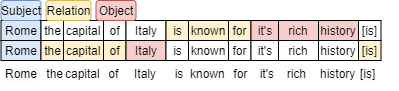
\includegraphics[width=8cm,height=1.5cm]{images/mlil/openie_example.png}
            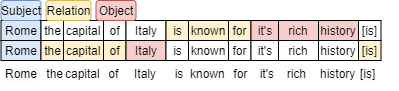
\includegraphics[width=0.8\hsize]{images/mlil/openie_example.png}
            \vspace*{-4ex}
            \caption{The extractions \textit{(Rome; [is] the capital of; Italy)} and \textit{(Rome; is known for; it's rich history)} can be seen as the output of the grid labeling. We additionally introduce a token \textit{[is]} to the input.}
            \label{fig:grid_example}
        \end{figure}

        We present a novel labelling-based architecture, \mlilboldlongname~(\mlilboldshortname), which models OpenIE as 2-D grid labeling problem of size $(M, N)$ where $M$ is a pre-defined maximum number of extractions and $N$ is the sentence length, as shown in Figure~\ref{fig:grid_example}.

        Each extraction corresponds to one row in the grid. Iterative assignment of labels in the grid helps \mlilshortname\ capture dependencies among extractions without the need for re-encoding. This makes it 25 times faster (80 sentences per second) than IMoJIE.

        While \mlilshortname\ gives high precision, we can further improve recall by incorporating (soft) global coverage constraints on this 2-D grid. We use constrained training \citep{mehta&al18} by adding a penalty term for all constraint violations. This encourages the model to satisfy these constraints during inference as well, leading to improved extraction quality, without affecting running time.


\section{Coordination Analyzer}

    Furthermore, the existing neural OpenIE models struggle in handling coordination structures, and do not split conjunctive extractions adequately. In response, we first design a new coordination analyzer \citep{ficler&goldberg16b}. It is built with the same \mlilshortname~ architecture, by interpreting each row in the 2-D grid as a coordination structure. This leads to a new state of the art on this task, with a 13 pt improvement in F1 over previous best reported result \citep{teranishi+19}, and a 2.5 pts gain in F1 over a strong BERT baseline. 

    We then combine the output of our coordination analyzer with our OpenIE system, resulting in a further increase in performance (Table~\ref{tab:redundancy-example}). We evaluate our final OpenIE system on four metrics from the literature and find that it exceeds in three of them by at least 4.2 pts in F1.
    
    We undertake manual evaluation to reaffirm the gains. Two annotators, blind to the underlying systems, independently label each extraction as correct or incorrect for a subset of 100 conjunctive sentences. Their inter-annotator agreement is 93.46\%. After resolving the extractions where they differ, we report the precision and yield in Table \ref{tab:manual_annotation}. Here, yield is the number of correct extractions generated by a system. It is a surrogate for recall, since its denominator, number of all correct extractions, is hard to annotate for OpenIE.  

    We find that \mlilshortname(CL)+CA significantly increases the yield (1.7x) compared to \mlilshortname(CL) at a marginal increase in precision. This result underscores the importance of splitting coordination structures for OpenIE. Our final OpenIE system, \mlilshortname(CL)+CA, is 25x faster than IMoJIE.

    \begin{table*}[h]
        \centering {\footnotesize
        \begin{tabular}{lccccccc}
        \toprule
        System                    
        & Precision & Yield & \makecell{Total\\Extrs}\\
        \midrule       
        \shortname(CL)
        & 77.9 & 131 & 174 \\
        \shortname(CL) + MLIL-CA
        & \textbf{78.8} & \textbf{222} & \textbf{291} \\
        \bottomrule
        \end{tabular}}
        \caption{Manual comparison of Precision and Yield on 100 random conjunctive sentences from CaRB Gold.}
        \label{tab:manual_annotation}
    \end{table*}

%%%%%%%%%%%%%%%%%%%%%%%%%%%%%%%%%%%%%%%%%%%%%%%%%%%%%%%%%%%%%%%%%%%%%%%%%%%%%%%%%%%%%%%%%%%%%%%%
% Uncategorised
%%%%%%%%%%%%%%%%%%%%%%%%%%%%%%%%%%%%%%%%%%%%%%%%%%%%%%%%%%%%%%%%%%%%%%%%%%%%%%%%%%%%%%%%%%%%%%%%



%%%%%%%%%%%%%%%%%%%%%%%%%%%%%%%%%%%%%%%%%%%%%%%%%%%%%%%%%%%%%%%%%%%%%%%%%%%%%%%%%%%%%%%%%%%%%%%%
% TABLES
%%%%%%%%%%%%%%%%%%%%%%%%%%%%%%%%%%%%%%%%%%%%%%%%%%%%%%%%%%%%%%%%%%%%%%%%%%%%%%%%%%%%%%%%%%%%%%%%

%%%%%%%%%%%%%%%%%%%%%%%%%%%%%%%%%%%%%%%%%%%%%%%%%%
% Milestones.

\chapter{Milestones of OpenIE}
\label{chap:milestones}
\input{sections/09.milestones.tex}

%%%%%%%%%%%%%%%%%%%%%%%%%%%%%%%%%%%%%%%%%%%%%%%%%%
% Future Ideas.

\chapter{Future Ideas}
\label{chap:future_ideas}
\section{OpenIE Milestones}

    This thesis covers several OpenIE milestones that mark our progress in the world of Open Information Extraction.

    \begin{enumerate}
        \item \textbf{Benchmark:} The problem of standardised and reliable benchmarking was solved using CaRB \citep{bhardwaj&al19}
        \item \textbf{Redundancy Removal:} \shortname \citep{kolluru&al20} and \mlilshortname\ have been able to produce non-redundant extractions
        \item \textbf{Variable Number of OpenIE tuples:} The iterative style architecture of \shortname\ and \mlilshortname\ overcome the problem of fixed number of extractions output by neural OpenIE systems using beam search.
        \item \textbf{Conjunction Splitting:} The MLIL-based Coordination Analyzer is now established as a new state-of-the-art.
        \item \textbf{Coreference Resolution:} Although OpenIE systems do resolve some coreferences, the problem is largely unsolved. It still requires careful attention and is left to future research.
        \item \textbf{Enhancing the Grammar of Extractions:} As neural systems lead to the rise of generative models in the OpenIE realm, generating grammatically correct extractions becomes increasingly vital. Improving the grammar of extractions has also been left to future research.
    \end{enumerate}


\section{Future Ideas}

    In the end, we contribute a few ideas to unravel interesting research directions that are yet unexplored.

    \begin{itemize}
        \item \textbf{Adding a language model to the extractor:} We have seen that the output extractions of generative OpenIE systems often do not lead to grammatical sentences when serialised. Adding a language model to the extractor seems to be a promising approach to tackle this issue.
        
        \item \textbf{Set Prediction Approach:} The task of OpenIE is inherently a set prediction task. The output needs to be a \emph{set} of OpenIE tuples. The order in which the tuples are spit out typically holds no significance. However, most of the OpenIE systems, including the state-of-the-art MLIL-based OpenIE as well as \shortname, treat it as sequence prediction task. The basic premise of the iterative architecture is also to predict a \emph{sequence-of-sequences}, rather than a \emph{set-of-sequences}. This violates the basic nature of the problem. Trying out set prediction techniques for OpenIE is a direction worth exploring. \cite{gao&al19} present a sequential set generation (SSG) framework which is a good point to start.
        
        \item \textbf{Optimally Ordering Training Data:} \cite{vinyals&al16} show that the order in which we arrange the input/output data significantly affects performance while learning an underlying model. While training OpenIE models, we arrange the input data based on its confidence score. However, multiple other orders are possible such as increasing order of tuple length. It will be interesting to study what affect does the order of training extractions have on the OpenIE models trained downstream. We might also derive cues to the optimal order for training OpenIE systems from here.
        
        \item \textbf{Incorporating CaRB's loss in \mlilshortname:} We can look for ways to incorporate the CaRB metric into the objective function of our model so that it can explicitly be optimised for. Even if this approach does not succeed in improving the OpenIE model, this experiment will reveal flaws in the metric used in our benchmark which we can use to improve our benchmark further.
    \end{itemize}

%%%%%%%%%%%%%%%%%%%%%%%%%%%%%%%%%%%%%%%%%%%%%%%%%%%%%%%%%%%%
% Appendices.

\appendix

\chapter{A SAMPLE APPENDIX}

\section{Performance of \shortname\ with varying sentence lengths}
    In this experiment, we measure the performance of baseline and our models by testing on sentences of varying lengths. We partition the original CaRB test data into 6 datasets with sentences of lengths (9-16 words), (17-24 words), (25-32 words), (33-40 words), (41-48 words) and (49-62 words) respectively. Note that the minimum and maximum sentence lengths are 9 and 62 respectively. We measure the Optimal F1 score of both Copy Attention + BERT and IMOJIE (Bootstrapped on OpenIE-4) on these partitions as depicted in Figure \ref{fig1}. \newline

    We observe that the performance deteriorates with increasing sentence length which is expected as well. Also, for each of the partitions, IMOJIE marginally performs better as compared to Copy Attention + BERT.

    \begin{figure}[h]
    \begin{center}
    \advance\leftskip-3cm
    \advance\rightskip-3cm
    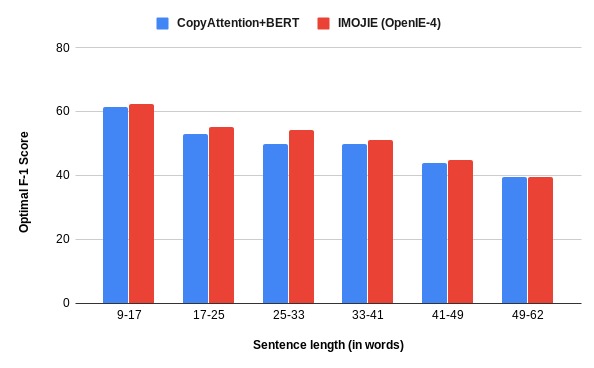
\includegraphics[keepaspectratio=true,scale=0.35]{images/imojie/Fig1.png}
    \caption{Measuring performance with varying input sentence lengths}
    \label{fig1}
    \end{center}
    \end{figure}
    
\section{Measuring Performance of \shortname\ on Varying Beam Size}
    We perform inference of the CopyAttention with BERT model on CaRB test set with beam sizes of 1, 3, 5, 7, and 11. We observe in Figure \ref{fig2} that AUC increases with increasing beam size. A system can surge its AUC by adding several low confidence tuples to its predicted set of tuples. This adds low precision - high recall points to the Precision-Recall curve of the system leading to higher AUC.\\
    On the other hand, Last F1 experiences a drop at very high beam sizes, thereby capturing the decline in performance. Optimal F1 saturates at high beam sizes since its calculation ignores the extractions below the optimal confidence threshold.\\
    This analysis also shows the importance of using Last F1 as a metric for measuring the performance of OpenIE systems.
    
    \begin{figure}
    \begin{center}
    \advance\leftskip-3cm
    \advance\rightskip-3cm
    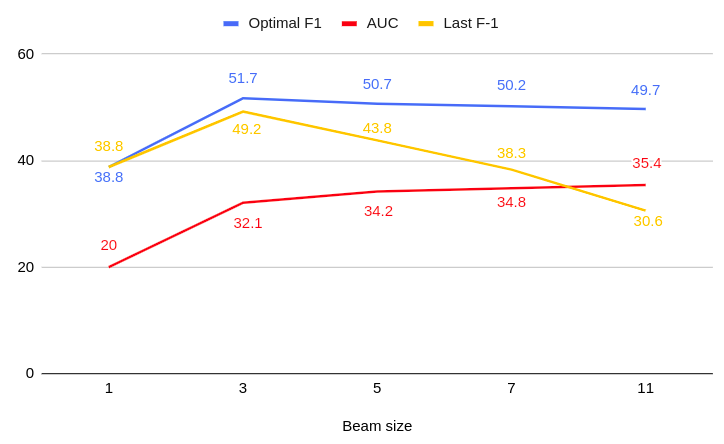
\includegraphics[keepaspectratio=true,width=\hsize]{images/imojie/Fig2.png}
    \caption{Measuring performance of CopyAttention with BERT model upon changing the beam size}
    \label{fig2}
    \end{center}
    \end{figure}
    
    \begin{table*}
    \begin{center} {\footnotesize
    \begin{tabular}{lccc}
    \hline
     \textbf{Model} & \multicolumn{3}{c}{\textbf{Dataset}}  \\
     & \multicolumn{1}{c}{Wire57} & \multicolumn{1}{c}{Penn} & \multicolumn{1}{c}{Web}\\
    \hline 
    CopyAttention + BERT & 45.60, \textbf{27.70}, 39.70 & 18.20, 7.9, 12.40 & 30.10, \textbf{18.00}, 14.60 \\ 
    \shortname & \textbf{46.20}, 26.60, \textbf{46.20} & \textbf{20.20}, \textbf{8.70}, \textbf{15.50} & \textbf{30.40}, 15.50, \textbf{26.40} \\ \hline
    \end{tabular} }
    \end{center}
    \caption{Evaluation on other datasets with the CaRB evaluation strategy}
    \label{tab:ODE}
    \end{table*}
    
\section{Evaluation of \shortname\ on other datasets}
    
    We use sentences from other benchmarks with the CaRB evaluation policy and we find similar improvements, as shown in Table \ref{tab:ODE}. \shortname{} consistently outperforms our strongest baseline, CopyAttention with BERT, over different test sets. This confirms that \shortname{} is domain agnostic.
    
\section{Visualizing Attention}
    \label{sec:visualize_attention}
    
    Attention has been used in a wide variety of settings to help the model learn to focus on important things \cite{bahdanau&al15, xu&al15, lu&al19}. However, the \shortname{} model is able to use attention to understand which words have already been generated, to focus on remaining words. In order to understand how the model achieves this, we visualize the learnt attention weights. There are two attention weights of importance, the learnt attention inside the BERT encoder and the attention between the decoder and encoder.  We use BertViz \cite{vig@19} to visualize the attention inside BERT.
    
    We consider the following sentence as the running example - "he served as the first prime minister of australia and became a founding justice of the high court of australia". We visualize the attention after producing the first extraction - ``he; served; as the first prime minister of australia''. Intuitively, we understand that the model must focus on the words ``founding'' and ``justice'' in order to generate the next extraction - ``he; became; a founding justice of the high court of australia''. In Figure \ref{fig:prime} and Figure \ref{fig:minister} (where the left-hand column contains the words which are used to attend while right-hand column contains the words which are attended over), we see that the words ``prime'' and ``minister'' of the original sentence have high attention over the same words in the first extraction. But the attention for ``founding'' and ``justice'' are limited to the original sentence.
    
    Based on these patterns, the decoder is able to give a high attention to the words ``founding'' and ``justice'' (as shown in Figure \ref{fig:att_weights}), in-order to successfully generate the second extraction "he; became; a founding justice of the high court of australia".
    
    \begin{figure}
    \begin{center}
    \advance\leftskip-3cm
    \advance\rightskip-3cm
    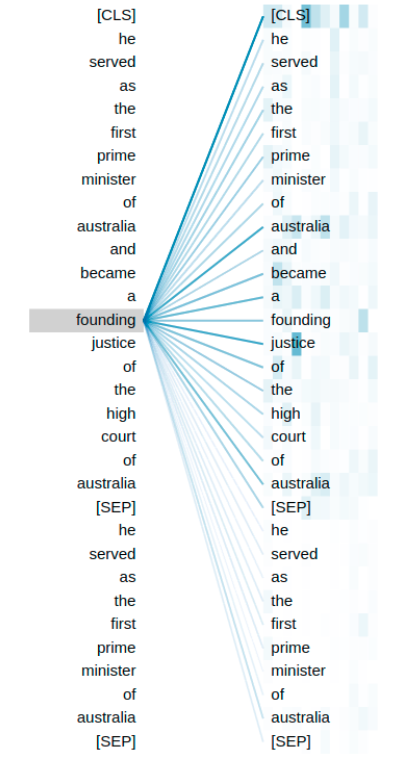
\includegraphics[keepaspectratio=true,width=0.5\vsize]{images/imojie/founding_cut.png}
    \caption{BERT attention for the word `founding'}
    \label{fig:founding}
    \end{center}
    \end{figure}
       
    \begin{figure}
    \begin{center}
    \advance\leftskip-3cm
    \advance\rightskip-3cm
    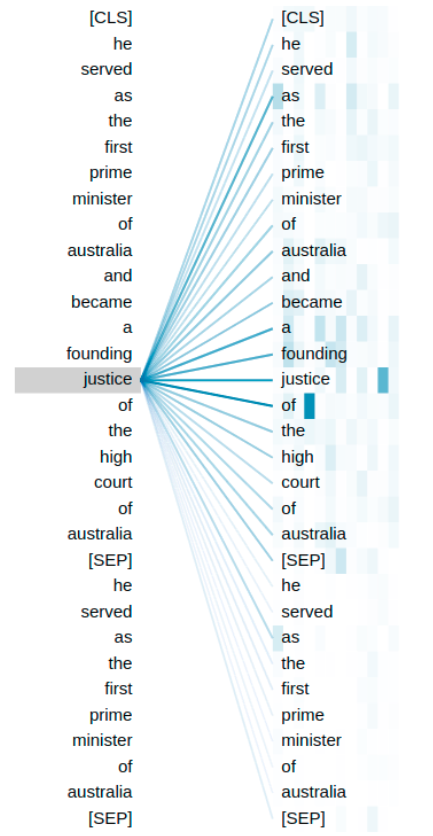
\includegraphics[keepaspectratio=true,width=0.5\hsize]{images/imojie/justice_cut.png}
    \caption{BERT attention for the word `justice'}
    \label{fig:justice}
    \end{center}
    \end{figure}
    
    \begin{figure}
    \begin{center}
    \advance\leftskip-3cm
    \advance\rightskip-3cm
    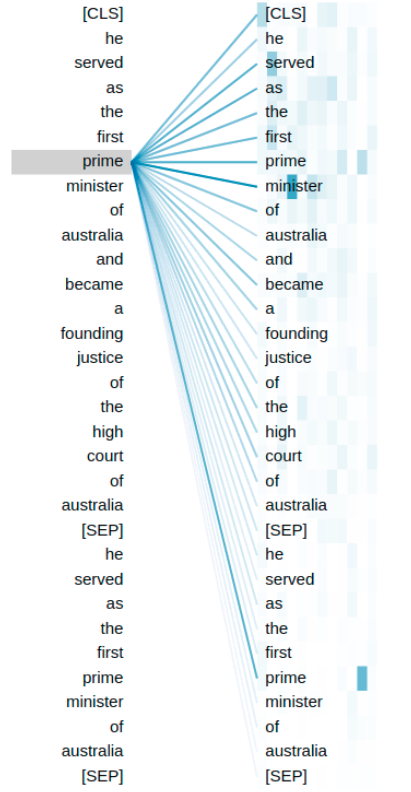
\includegraphics[keepaspectratio=true,width=0.5\hsize]{images/imojie/prime_cut.png}
    \caption{BERT attention for the word `prime'}
    \label{fig:prime}
    \end{center}
    \end{figure}
    
    \begin{figure}
    \begin{center}
    \advance\leftskip-3cm
    \advance\rightskip-3cm
    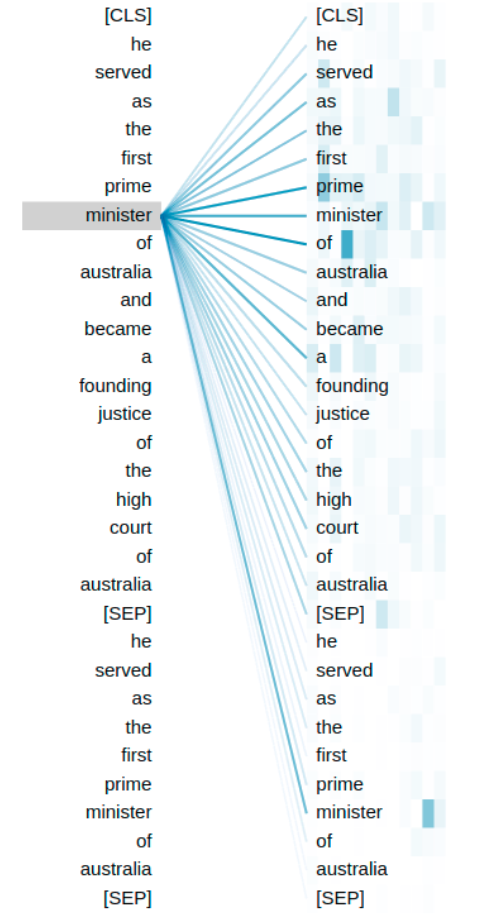
\includegraphics[keepaspectratio=true,width=0.5\hsize]{images/imojie/minister_cut.png}
    \caption{BERT attention for the word `minister'}
    \label{fig:minister}
    \end{center}
    \end{figure}
    
    \begin{figure*}
    \begin{center}
    \advance\leftskip-3cm
    \advance\rightskip-3cm
    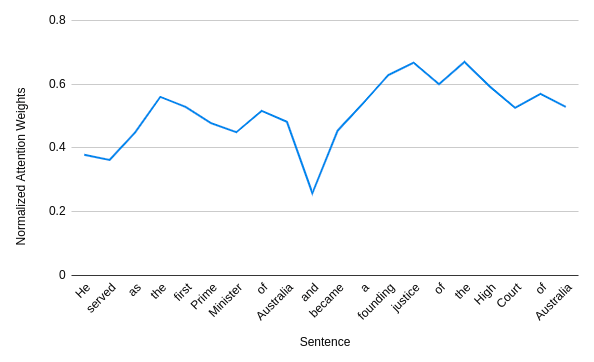
\includegraphics[keepaspectratio=true,width=\hsize]{images/imojie/att_weights.png}
    \caption{Attention weights for the decoder}
    \label{fig:att_weights}
    \end{center}
    \end{figure*}

%%%%%%%%%%%%%%%%%%%%%%%%%%%%%%%%%%%%%%%%%%%%%%%%%%%%%%%%%%%%
% Bibliography.

\begin{singlespace}
  \bibliography{refs}
  \bibliographystyle{acl_natbib}
\end{singlespace}

%%%%%%%%%%%%%%%%%%%%%%%%%%%%%%%%%%%%%%%%%%%%%%%%%%%%%%%%%%%%
% List of papers

\listofpapers
\begin{enumerate}
    \item Authors....  \newblock
     Title...
      \newblock {\em Journal}, Volume,
      Page, (year).
    \item Authors....  \newblock
      Title...
       \newblock {\em Journal}, Volume,
       Page, (year).
\end{enumerate}

\end{document}
